% ============================================================
%  宽松风险平价答辩 PPT
%  编译：xelatex rrp_defense.tex  →  rrp_defense.pdf
%  位置：report/defense_ppt/
%  图片：../../results/figures/（相对于本文件）
% ============================================================
\documentclass[aspectratio=169,11pt]{beamer}
\usepackage{beamerthemeSWUFE}
\usepackage{booktabs}
\usepackage{amsmath}
\usepackage{array}
\usepackage{colortbl}

% 图片搜索路径：results/figures 和本地 logo
\graphicspath{{../../results/figures/}{assets/logos/}}

% ── 封面信息 ─────────────────────────────────────────────────────────────────
\title{宽松风险平价在全球 ETF\\资产配置中的改进与实证研究}
\subtitle{本科毕业论文答辩}
\author{许哲圣}
\studentid{42353012}
\school{特拉华数据科学学院}
\major{金融数学（量化分析方向）}
\supervisor{王磊}
\date{2026年5月}

% ── 数值宏（全部来自 generated_numbers.tex）──────────────────────────────────
\newcommand{\etfCount}{30}
\newcommand{\evalStartDate}{2019-01-01}
\newcommand{\evalEndDate}{2026-05-29}
\newcommand{\evalMonths}{89}
\newcommand{\txCostBps}{3}
\newcommand{\riskFreeRate}{1.82\%}
\newcommand{\dataFirstDate}{2018-02-28}
% Global RRP
\newcommand{\globalNetReturn}{4.59\%}
\newcommand{\globalVolatility}{4.11\%}
\newcommand{\globalSharpe}{0.674}
\newcommand{\globalSortino}{0.770}
\newcommand{\globalMaxDD}{-7.14\%}
\newcommand{\globalMonthlyTurnover}{22.30\%}
% Convex Adaptive
\newcommand{\convexNetReturn}{6.80\%}
\newcommand{\convexVolatility}{5.21\%}
\newcommand{\convexSharpe}{0.956}
\newcommand{\convexSortino}{1.468}
\newcommand{\convexMaxDD}{-6.66\%}
\newcommand{\convexMonthlyTurnover}{1.24\%}
% Improved Convex（主模型）
\newcommand{\improvedNetReturn}{5.57\%}
\newcommand{\improvedVolatility}{2.62\%}
\newcommand{\improvedSharpe}{1.431}
\newcommand{\improvedSortino}{2.099}
\newcommand{\improvedMaxDD}{-3.95\%}
\newcommand{\improvedCalmar}{1.410}
\newcommand{\improvedMonthlyTurnover}{2.07\%}
% HERC
\newcommand{\hercNetReturn}{2.23\%}
\newcommand{\hercVolatility}{0.57\%}
\newcommand{\hercSharpe}{0.718}
\newcommand{\hercSortino}{1.053}
\newcommand{\hercMaxDD}{-0.58\%}
% 等权 / 60-40
\newcommand{\equalNetReturn}{10.66\%}
\newcommand{\equalSharpe}{0.798}
\newcommand{\equalSortino}{1.276}
\newcommand{\equalMaxDD}{-13.91\%}
\newcommand{\sixtyFortyNetReturn}{8.02\%}
\newcommand{\sixtyFortySharpe}{0.695}
\newcommand{\sixtyFortySortino}{1.119}
\newcommand{\sixtyFortyMaxDD}{-14.71\%}
% Walk-forward
\newcommand{\wfSharpeMean}{1.116}
\newcommand{\wfSharpeMedian}{1.014}
\newcommand{\wfReturnMean}{7.18\%}
\newcommand{\wfReturnMedian}{6.37\%}
\newcommand{\wfDDMean}{-2.07\%}
% 统计检验
\newcommand{\improvedVsGlobalDiff}{0.757}
\newcommand{\improvedVsGlobalPValue}{0.004}

% ── 辅助命令：图片帧（单图 + 可选注释）────────────────────────────────────────
% \figframe{帧标题}{文件名}{宽度比}{说明文字（空=不显示）}
\newcommand{\figframe}[4]{%
  \begin{frame}{#1}
    \begin{center}
      \includegraphics[width=#3\textwidth,height=0.68\textheight,keepaspectratio]{#2}
    \end{center}
    \begin{center}\footnotesize #4\end{center}
  \end{frame}%
}

\begin{document}

% ════════════════════════════════════════════════════════════════════════════
\begin{frame}\titlepage\end{frame}

\begin{frame}{目录}\tableofcontents\end{frame}

% ════════════════════════════════════════════════════════════════════════════
\section{研究背景与意义}
% ════════════════════════════════════════════════════════════════════════════

\begin{frame}{长期配置的核心挑战}
  \begin{columns}[T]
    \begin{column}{0.48\textwidth}
      \textbf{为什么不能直接用均值—方差？}
      \begin{itemize}
        \item Michaud（1989）：收益率估计误差约为协方差的 \textbf{10 倍}，微小扰动导致权重剧烈漂移
        \item DeMiguel 等（2009）：14 种优化策略均未稳定击败 1/N 等权组合
        \item 实务上：收益率预测本身高度不确定，机构更需要\textbf{风险可归因}的框架
      \end{itemize}
      \vspace{0.4em}
      \textbf{全球 ETF 落地的三重难题}
      \begin{itemize}
        \item 相关结构\textbf{时变}，固定窗口协方差估计滞后
        \item 严格 ERC + 组别上限 + CVaR → \textbf{非凸}，难以统一求解
        \item 月频调仓 × \txCostBps{} bps 成本 × 长周期 → \textbf{净收益侵蚀}明显
      \end{itemize}
    \end{column}
    \begin{column}{0.48\textwidth}
      \begin{block}{风险平价的核心逻辑}
        \centering\large
        $RC_i = w_i \cdot \dfrac{(\Sigma w)_i}{\sigma_p}$\\[0.5em]
        \normalsize 目标：$RC_i = b_i \cdot \sigma_p$\\[0.3em]
        \small 以\textbf{风险贡献}替代资金金额分配\\
        对收益预测依赖低，逻辑清晰
      \end{block}
      \vspace{0.4em}
      \begin{alertblock}{本文的解法}
        宽松 RRP + CVaR 尾部约束 +\\
        $\ell_1$ 换手惩罚 →\\
        \textbf{统一可稳定求解的凸优化框架}
      \end{alertblock}
    \end{column}
  \end{columns}
\end{frame}

\begin{frame}{研究问题与研究思路}
  \begin{columns}[T]
    \begin{column}{0.50\textwidth}
      \textbf{四个核心问题}
      \begin{enumerate}
        \item 宽松风险平价能否在 \etfCount{} 支全球 ETF 中建立\textbf{风险来源清晰}的配置框架？
        \item 加入 CVaR 约束和换手惩罚后，\textbf{收益、回撤与换手}三维权衡是否确实改善？
        \item HERC 等层次化基准在同一样本中\textbf{表现如何}，与主模型是何关系？
        \item 稳健性检验能否识别结论对\textbf{样本期和参数}的依赖程度？
      \end{enumerate}
    \end{column}
    \begin{column}{0.47\textwidth}
      \textbf{研究路径}
      \begin{itemize}
        \item[\textcolor{swufeGold}{$\triangleright$}] 梳理 MV → 风险预算 → CVaR → HRP 的理论联系
        \item[\textcolor{swufeGold}{$\triangleright$}] 构建可交易 ETF 资产池与统一回测标准
        \item[\textcolor{swufeGold}{$\triangleright$}] 相同设计下横向对比四个模型
        \item[\textcolor{swufeGold}{$\triangleright$}] 多维度稳健性检验 + 过拟合诊断约束结论范围
      \end{itemize}
      \vspace{0.5em}
      \begin{block}{评价窗口}
        \centering\small
        \evalStartDate{} — \evalEndDate{}\\
        \evalMonths{} 个月度观察点\\
        单边成本 \txCostBps{} bps，全程无前视
      \end{block}
    \end{column}
  \end{columns}
\end{frame}

\begin{frame}{三项边际贡献}
  \begin{swufekeypoints}
    \swufepoint{数据层}{01}{以\textbf{可交易 ETF} 替代不可交易指数，回测成本与权重更贴近真实执行——而非停留在指数层面，使"能不能做到"这一问题有了直接的答案}
    \swufepoint{方法层}{02}{将风险预算偏离惩罚、CVaR 约束、$\ell_1$ 换手惩罚和资产组上限\textbf{统一纳入}同一凸优化框架，允许同时处理多个实施约束而无需逐一妥协}
    \swufepoint{验证层}{03}{串联子区间、参数扰动、协方差估计、过拟合诊断等多种稳健性检验，将结论\textbf{明确限定}在具体样本区间与参数设定，避免过度外推}
  \end{swufekeypoints}
\end{frame}

% ════════════════════════════════════════════════════════════════════════════
\section{文献综述与理论基础}
% ════════════════════════════════════════════════════════════════════════════

\begin{frame}[shrink=3]{从均值—方差到风险预算：理论脉络}
  \begin{columns}[T]
    \begin{column}{0.50\textwidth}
      \textbf{均值—方差与估计误差}
      \begin{itemize}
        \item Markowitz（1959）：奠基，二次规划
        \item Jorion（1986）：Bayes-Stein 收缩量化参数不确定性
        \item \alert{共同结论}：收益预测不确定性高，\textbf{难以持续击败简单基准}
      \end{itemize}
      \vspace{0.35em}
      \textbf{协方差估计进展}
      \begin{itemize}
        \item 随机矩阵理论（Laloux 1999）：大量特征值为噪声
        \item CM-IEWMA（Johansson 2023）：凸组合多个 EWMA 估计器
        \item 端到端深度学习（Bongiorno 2025）：优越但\alert{难纳入硬约束}
      \end{itemize}
    \end{column}
    \begin{column}{0.47\textwidth}
      \textbf{风险平价与宽松风险预算}
      \begin{itemize}
        \item Qian（2005）：风险贡献平等 = 最优分散
        \item Maillard 等（2010）：ERC 唯一性证明
        \item Gambeta \& Kwon（2020）：\textbf{宽松 RRP} 数学性质
      \end{itemize}
      \vspace{0.35em}
      \textbf{层次化方法}
      \begin{itemize}
        \item HRP（López de Prado 2016）：层次聚类，回避矩阵求逆
        \item HERC（Raffinot 2018）：簇间引入风险贡献逻辑
        \item \alert{共同局限}：难以直接纳入 CVaR 和换手惩罚
      \end{itemize}
    \end{column}
  \end{columns}
\end{frame}

\begin{frame}{CVaR 约束与交易成本的理论依据}
  \begin{columns}[T]
    \begin{column}{0.52\textwidth}
      \textbf{CVaR 的凸性与线性重表述}\\[0.3em]
      Rockafellar \& Uryasev（2000；2002）：
      \[
        \mathrm{CVaR}_\alpha(w) = \min_\eta \Bigl[\eta + \tfrac{1}{(1-\alpha)T}
        \textstyle\sum_t\max(-r_t^\top w - \eta,\, 0)\Bigr]
      \]
      \begin{itemize}
        \item 次可加性 + 凸性：\textbf{天然适合约束优化}
        \item 引入辅助变量 $\eta$ 后等价为\textbf{线性不等式组}
        \item 与 $\ell_1$ 换手惩罚可统一在同一 QP/SOCP 框架
      \end{itemize}
    \end{column}
    \begin{column}{0.45\textwidth}
      \textbf{交易成本建模}\\[0.3em]
      Almgren \& Chriss（2001）：换手速率与市场冲击的根本张力
      \vspace{0.4em}
      \begin{block}{本文：线性成本近似}
        \centering
        $\mathrm{TC}_t = c \cdot \|w_t - w_{t-1}^+\|_1$\\[0.3em]
        \small $c = \txCostBps$ bps 单边\\月频调仓下误差可控
      \end{block}
      \vspace{0.4em}
      \small \textbf{国内研究（华泰 2020—2024）指出}：低利率环境下换手成本是风险平价落地的核心约束，月频再平衡的成本积累不可忽视
    \end{column}
  \end{columns}
\end{frame}

% ════════════════════════════════════════════════════════════════════════════
\section{理论框架与模型方法}
% ════════════════════════════════════════════════════════════════════════════

\begin{frame}{从严格 ERC 到宽松风险平价}
  \begin{columns}[T]
    \begin{column}{0.46\textwidth}
      \textbf{标准风险平价（ERC）}\\[0.2em]
      风险贡献：$RC_i = w_i \cdot \dfrac{(\Sigma w)_i}{\sigma_p}$\\[0.4em]
      严格等式约束：$RC_i = b_i \sigma_p$\\[0.4em]
      \alert{困难}：同时加权重上下限、资产组约束后，等式约束使问题\textbf{非凸}，标准求解器无法直接处理

      \vspace{0.6em}
      \textbf{宽松 RRP：严格等式 → 偏离惩罚}
      \[
        \min_w \sum_i \!\Bigl(\tfrac{RC_i}{\sigma_p} - b_i\Bigr)^{\!2}
        + \lambda_{\text{reg}}\|w - w_0\|_2^2
      \]
      允许可量化的预算偏离，换取约束灵活性
    \end{column}
    \begin{column}{0.51\textwidth}
      \textbf{Convex Adaptive Global RRP}\\[0.3em]
      将风险预算思想凸化，统一纳入多个约束：
      \small
      \begin{align*}
        \min_w\; J(w)
          &= \underbrace{\lambda_v w^\top\Sigma_t w}_{\text{波动率项}}
           + \underbrace{\lambda_b\|w - b_t\|_2^2}_{\text{预算偏离}} \\[2pt]
          &\;+ \underbrace{\lambda_{to}\|w - w_{t-1}^+\|_1}_{\text{换手惩罚}}
           + \underbrace{\lambda_c\,\mathrm{CVaR}_\alpha(w)}_{\text{尾部约束}}
           - \underbrace{\lambda_r\,\mu_t^\top w}_{\text{收益奖励}}
      \end{align*}
      \normalsize
      \vspace{0.1em}
      约束集：$\sum_i w_i=1,\ 0\le w_i\le u_i,\ L_g\le\sum_{i\in g}w_i\le U_g$
    \end{column}
  \end{columns}
\end{frame}

\begin{frame}{四模型定位与参数冻结策略}
  \begin{columns}[T]
    \begin{column}{0.54\textwidth}
      \renewcommand{\arraystretch}{1.3}
      \footnotesize
      \begin{tabular}{@{}l>{\raggedright\arraybackslash}p{4.0cm}l@{}}
        \toprule
        模型 & 核心特征 & 角色 \\
        \midrule
        Global RRP & 基准宽松风险预算，无换手约束 & 出发点 \\
        Convex Adaptive & $\ell_1$ 换手惩罚 + 资产组上限 & 降换手 \\
        \textbf{Improved Convex} & \textbf{+ CVaR 约束 + 参数冻结} & \textbf{主模型} \\
        HERC & 层次聚类递归分配，无凸优化 & 层次化基准 \\
        \bottomrule
      \end{tabular}
      \vspace{0.4em}
      \footnotesize
      所有模型：长仓、权重归一、月度调仓、\\
      滚动估计、扣除 \txCostBps{} bps 单边成本
    \end{column}
    \begin{column}{0.43\textwidth}
      \begin{block}{参数冻结：防止过拟合的关键}
        \footnotesize
        \begin{enumerate}
          \item 在\textbf{训练集}内网格搜索超参数候选
          \item 筛选 OOS 期稳健的候选集（candidate\_23）
          \item \textbf{冻结参数}后在完整 \evalStartDate{}—\evalEndDate{} 重跑
          \item 所有报告数字均来自冻结参数下的结果
        \end{enumerate}
      \end{block}
      \vspace{0.3em}
      \footnotesize
      \begin{tabular}{@{}ll@{}}
        历史窗口 & 252 交易日 \\
        协方差估计 & EWMA \\
        单资产最大权重 & 45\% \\
        换手上限 & 80\% \\
        CVaR 置信水平 & 95\% \\
      \end{tabular}
    \end{column}
  \end{columns}
\end{frame}

% ════════════════════════════════════════════════════════════════════════════
\section{数据与回测设计}
% ════════════════════════════════════════════════════════════════════════════

\begin{frame}{\etfCount{} 支全球 ETF：8 大风险来源（来自 src/asset\_universe.py）}
  \footnotesize
  \renewcommand{\arraystretch}{1.15}
  \begin{columns}[T]
    \begin{column}{0.50\textwidth}
      \begin{tabular}{@{}lll@{}}
        \toprule
        类别 & 代表品种 & 数量 \\
        \midrule
        债券 & 国债、信用债、可转债、货币 & 4 \\
        A 股宽基 & 沪深 300/500/1000、创业板、红利 & 5 \\
        中国科技 & 半导体、AI、机器人、新能源 & 7 \\
               & 中韩半导体、科创 50、云计算 & \\
        \bottomrule
      \end{tabular}
    \end{column}
    \begin{column}{0.48\textwidth}
      \begin{tabular}{@{}lll@{}}
        \toprule
        类别 & 代表品种 & 数量 \\
        \midrule
        行业与消费 & 证券、军工、消费 & 3 \\
        港股与贵金属 & 恒生、白银 LOF & 2 \\
        全球股票 & 纳指、标普 500、日经、欧洲 & 4 \\
        大宗商品 & 黄金、有色、豆粕、煤炭、原油 & 5 \\
        \bottomrule
      \end{tabular}
      \vspace{0.4em}
      \small
      数据起始 \dataFirstDate{}（含训练期）\\
      评价区间 \evalStartDate{}—\evalEndDate{}\\
      共 \evalMonths{} 个月度观察点
    \end{column}
  \end{columns}
\end{frame}

\figframe{因子暴露结构：各 ETF 对主要风险因子的敞口}{asset_pricing_factor_exposure.png}{0.90}{}

\begin{frame}{静态权重演进：从国内到全球多资产}
  \begin{columns}[T]
    \begin{column}{0.32\textwidth}
      \centering
      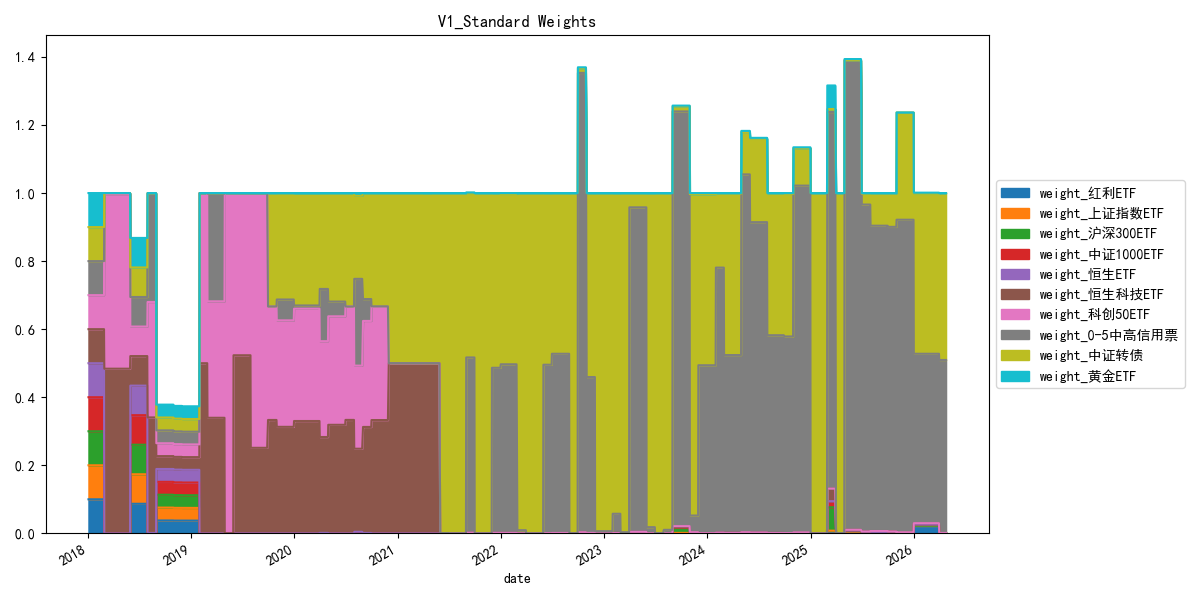
\includegraphics[width=\textwidth,height=0.60\textheight,keepaspectratio]{static_v1_standard_weights.png}\\[0.3em]
      \footnotesize \textbf{标准风险平价}\\债券主导，高集中度
    \end{column}
    \begin{column}{0.32\textwidth}
      \centering
      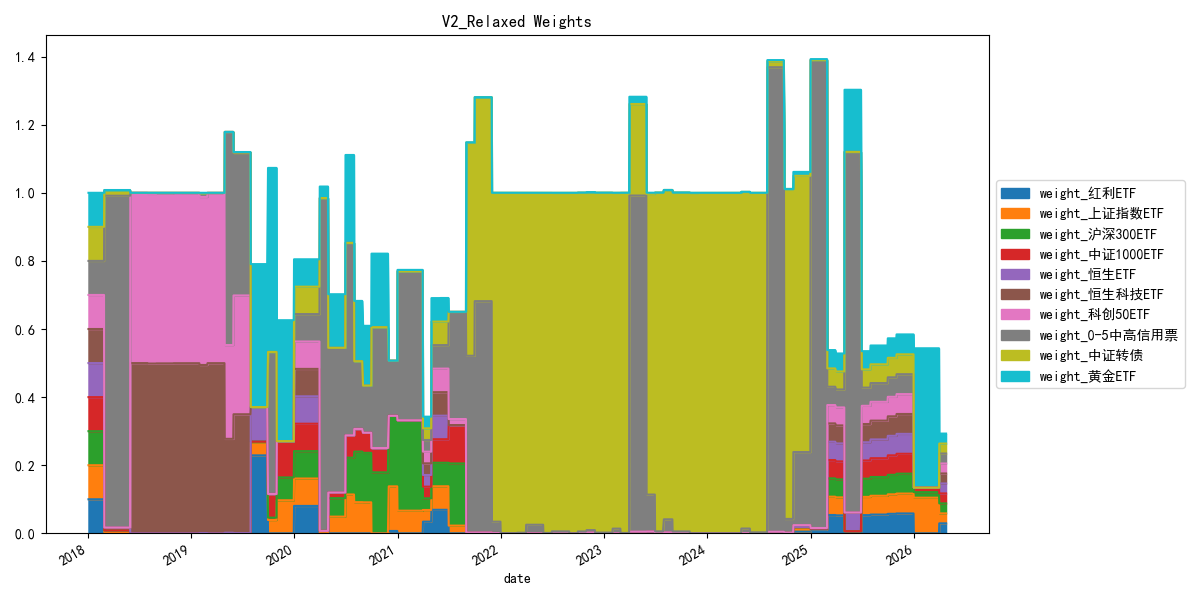
\includegraphics[width=\textwidth,height=0.60\textheight,keepaspectratio]{static_v2_relaxed_weights.png}\\[0.3em]
      \footnotesize \textbf{宽松 RRP}\\偏离惩罚引入，权重更分散
    \end{column}
    \begin{column}{0.32\textwidth}
      \centering
      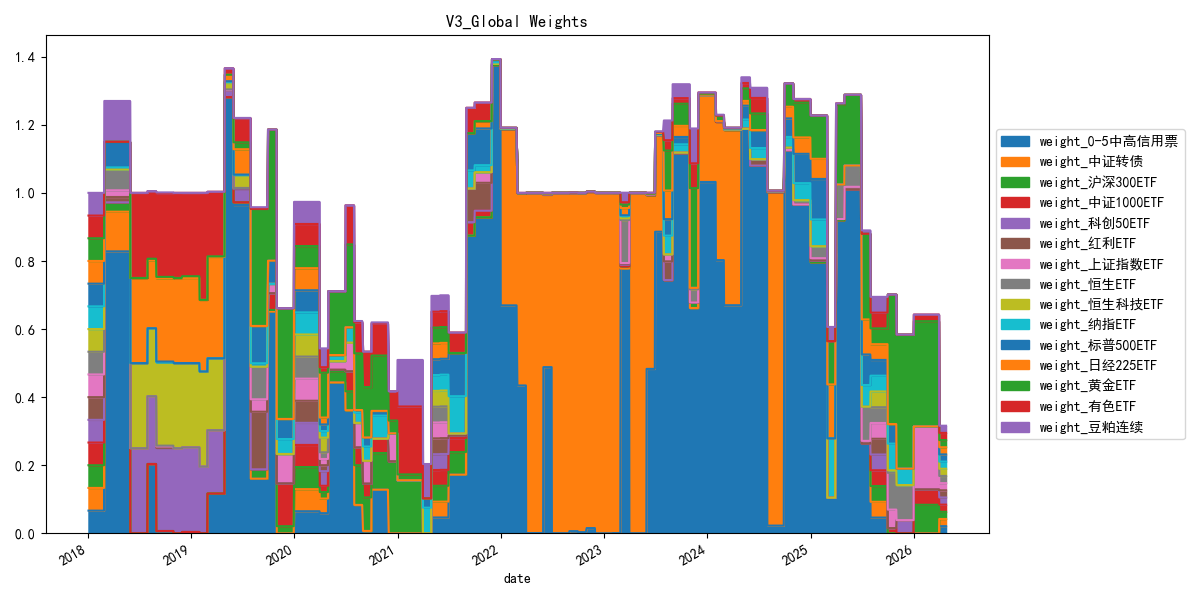
\includegraphics[width=\textwidth,height=0.60\textheight,keepaspectratio]{static_v3_global_weights.png}\\[0.3em]
      \footnotesize \textbf{Global RRP（30 支）}\\跨 8 大类，结构更均衡
    \end{column}
  \end{columns}
\end{frame}

% ════════════════════════════════════════════════════════════════════════════
\section{实证结果与分析}
% ════════════════════════════════════════════════════════════════════════════

\begin{frame}{绩效汇总：\evalStartDate{}—\evalEndDate{}，\evalMonths{} 个月度观察点}
  \footnotesize
  \renewcommand{\arraystretch}{1.3}
  \begin{center}
    \begin{tabular}{@{}lccccc@{}}
      \toprule
      模型 & 净年化收益 & Sharpe & Sortino & 最大回撤 & 月均换手 \\
      \midrule
      Global RRP      & \globalNetReturn  & \globalSharpe  & \globalSortino  & \globalMaxDD  & \globalMonthlyTurnover \\
      Convex Adaptive & \convexNetReturn  & \convexSharpe  & \convexSortino  & \convexMaxDD  & \convexMonthlyTurnover \\
      \rowcolor{swufeLight}
      \textbf{Improved Convex} & \textbf{\improvedNetReturn} & \textbf{\improvedSharpe} & \textbf{\improvedSortino} & \textbf{\improvedMaxDD} & \textbf{\improvedMonthlyTurnover} \\
      HERC            & \hercNetReturn    & \hercSharpe    & \hercSortino    & \hercMaxDD    & 5.78\% \\
      \midrule
      等权基准        & \equalNetReturn   & \equalSharpe   & \equalSortino   & \equalMaxDD   & 1.24\% \\
      60/40 基准      & \sixtyFortyNetReturn & \sixtyFortySharpe & \sixtyFortySortino & \sixtyFortyMaxDD & 1.43\% \\
      \bottomrule
    \end{tabular}
  \end{center}
  \vspace{0.2em}
  \scriptsize 无风险利率 \riskFreeRate{}；净年化收益已扣除 \txCostBps{} bps 单边成本
\end{frame}

\begin{frame}{净值路径：全模型对比}
  \begin{center}
    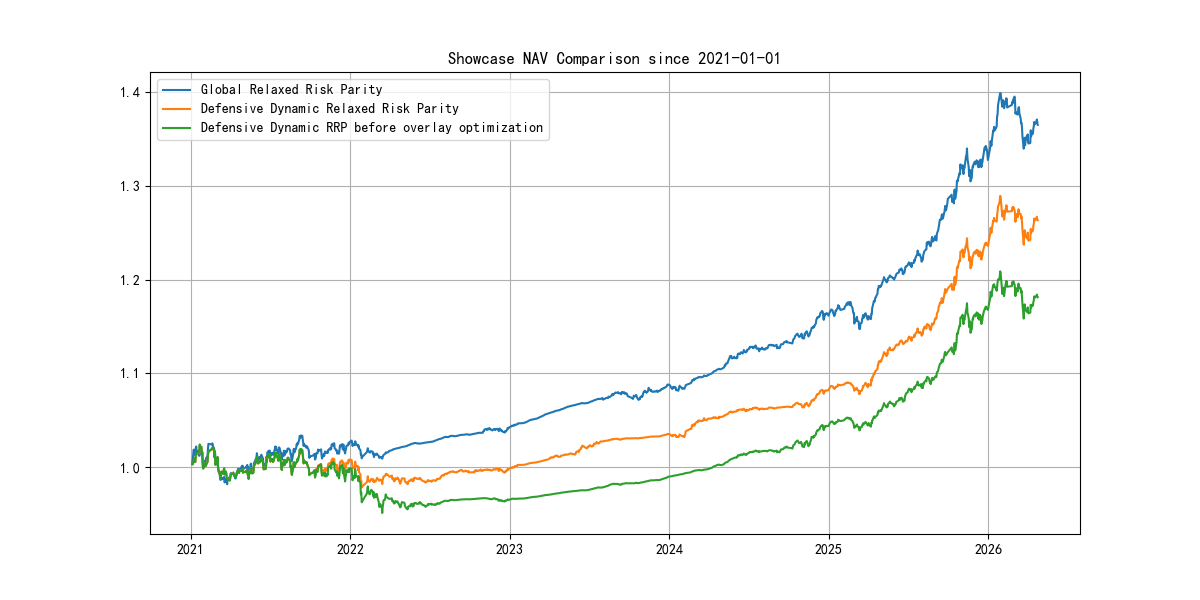
\includegraphics[width=0.88\textwidth,height=0.64\textheight,keepaspectratio]{showcase_nav_comparison.png}
  \end{center}
  \vspace{-0.2em}
  \begin{columns}[T]
    \begin{column}{0.50\textwidth}
      \footnotesize
      \begin{itemize}
        \item \textbf{Improved Convex} 净值稳步攀升，波动远低于等权/60-40
      \end{itemize}
    \end{column}
    \begin{column}{0.50\textwidth}
      \footnotesize
      \begin{itemize}
        \item \textbf{HERC} 近乎横盘——反映其实质是近全仓债券，非多资产分散
      \end{itemize}
    \end{column}
  \end{columns}
\end{frame}

\begin{frame}{回撤路径：全模型对比}
  \begin{center}
    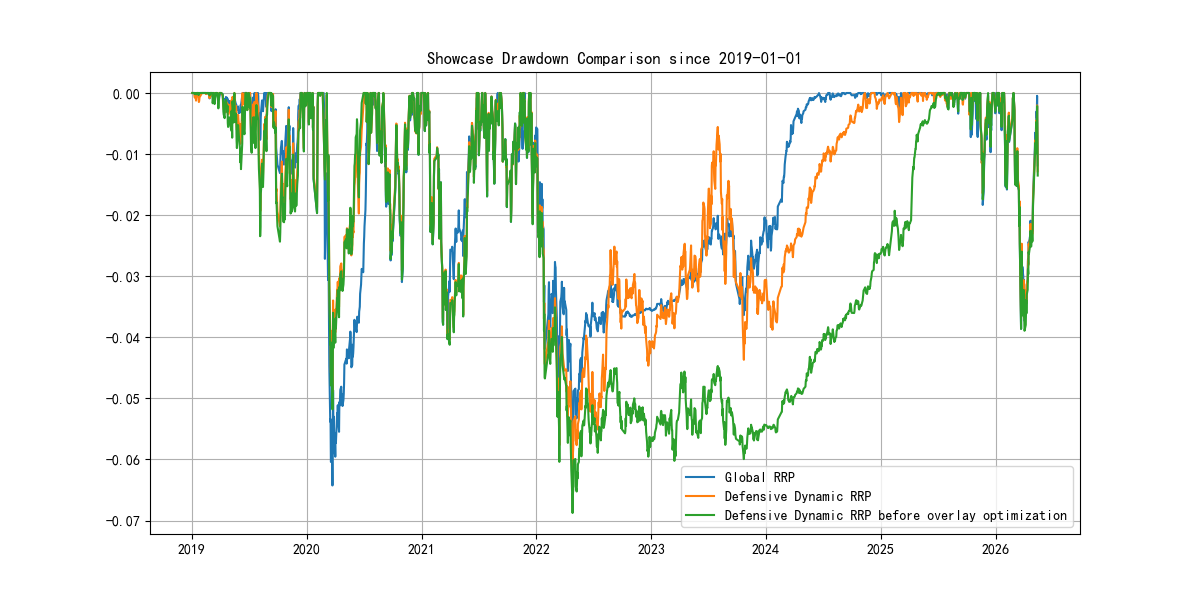
\includegraphics[width=0.88\textwidth,height=0.64\textheight,keepaspectratio]{showcase_drawdown_comparison.png}
  \end{center}
  \vspace{-0.2em}
  \begin{columns}[T]
    \begin{column}{0.50\textwidth}
      \footnotesize
      \begin{itemize}
        \item Improved Convex 最大回撤 \improvedMaxDD{}，显著优于等权 \equalMaxDD{} 和 60/40 \sixtyFortyMaxDD{}
      \end{itemize}
    \end{column}
    \begin{column}{0.50\textwidth}
      \footnotesize
      \begin{itemize}
        \item Global RRP 回撤 \globalMaxDD{}，换手高（\globalMonthlyTurnover{}）是主要拖累
      \end{itemize}
    \end{column}
  \end{columns}
\end{frame}

\begin{frame}{静态基准 vs 动态模型：净值演进}
  \begin{center}
    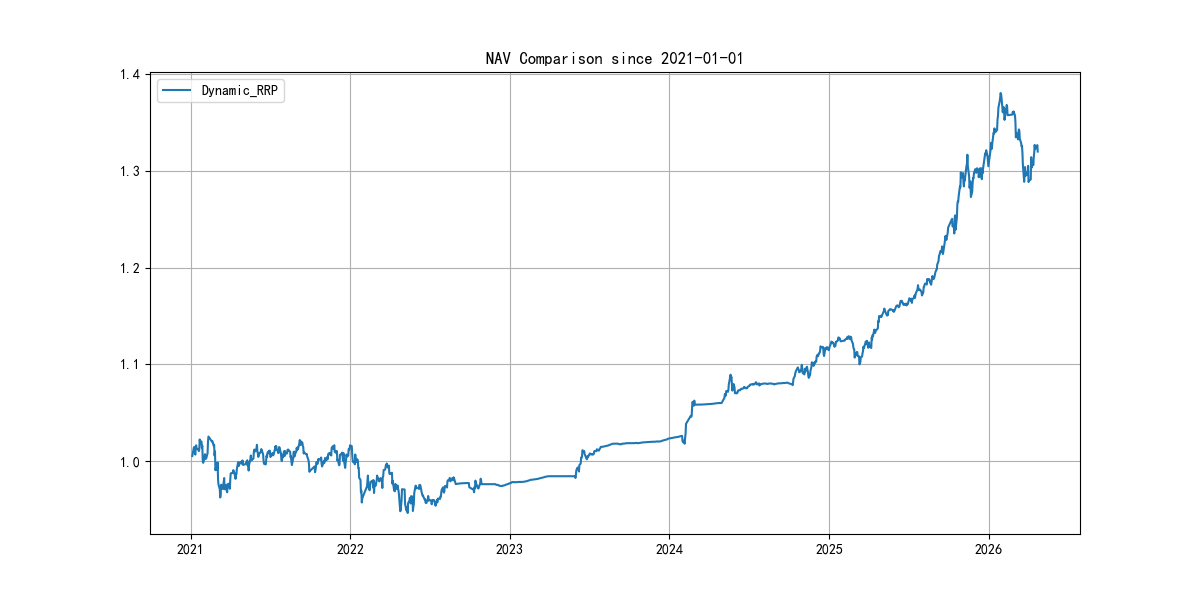
\includegraphics[width=0.88\textwidth,height=0.66\textheight,keepaspectratio]{static_vs_dynamic_nav.png}
  \end{center}
  \vspace{-0.2em}
  \footnotesize\centering
  动态调仓（滚动协方差 + 月度再平衡）相比单期静态权重有明显的净值优势，说明时变相关结构值得跟踪
\end{frame}

\begin{frame}{Convex 系列对比：净值与回撤}
  \begin{columns}[T]
    \begin{column}{0.50\textwidth}
      \centering
      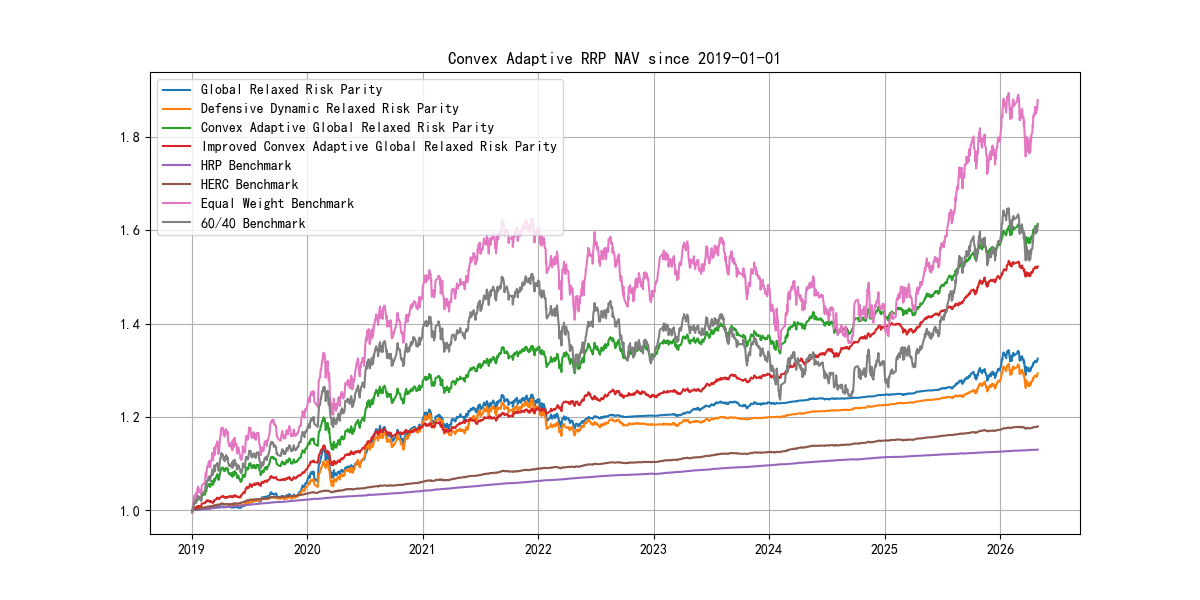
\includegraphics[width=\textwidth,height=0.66\textheight,keepaspectratio]{convex_adaptive_nav_comparison.png}\\
      \footnotesize\centering 净值路径
    \end{column}
    \begin{column}{0.50\textwidth}
      \centering
      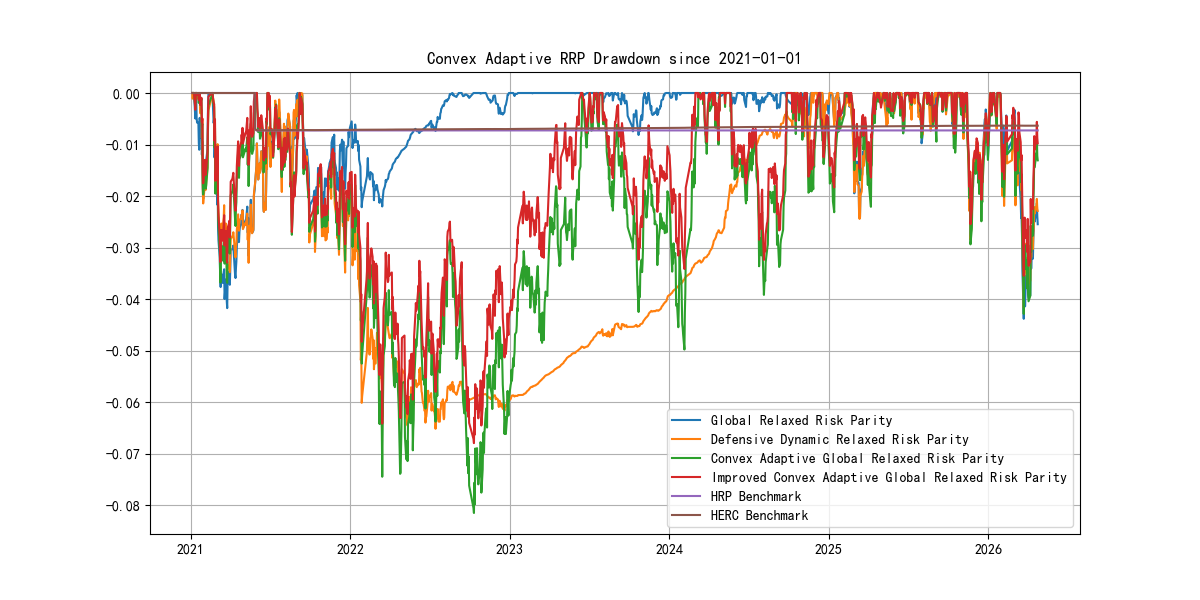
\includegraphics[width=\textwidth,height=0.66\textheight,keepaspectratio]{convex_adaptive_drawdown_comparison.png}\\
      \footnotesize\centering 回撤路径
    \end{column}
  \end{columns}
  \vspace{0.2em}
  \footnotesize\centering
  从 Global RRP → Convex Adaptive → Improved Convex：净值更稳，回撤更浅，换手逐步压缩
\end{frame}

\begin{frame}{换手率对比：CVaR + 惩罚项的实际效果}
  \begin{center}
    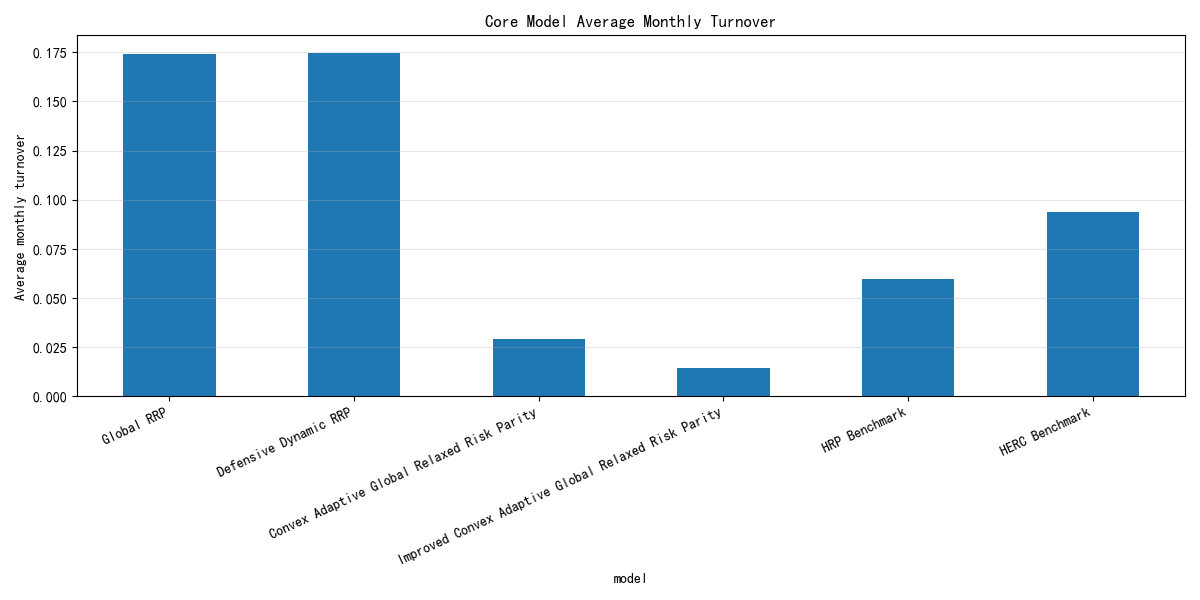
\includegraphics[width=0.88\textwidth,height=0.64\textheight,keepaspectratio]{convex_adaptive_turnover_comparison.png}
  \end{center}
  \vspace{-0.2em}
  \begin{columns}[T]
    \begin{column}{0.50\textwidth}
      \footnotesize
      \begin{itemize}
        \item Global RRP 月均换手 \globalMonthlyTurnover{} → Improved Convex 压至 \textbf{\improvedMonthlyTurnover}，降幅约 \textbf{10 倍}
      \end{itemize}
    \end{column}
    \begin{column}{0.50\textwidth}
      \footnotesize
      \begin{itemize}
        \item 换手大幅下降后成本拖累消失，净 Sharpe 从 \globalSharpe{} 升至 \improvedSharpe{}
      \end{itemize}
    \end{column}
  \end{columns}
\end{frame}

\begin{frame}{交易成本拖累对比}
  \begin{center}
    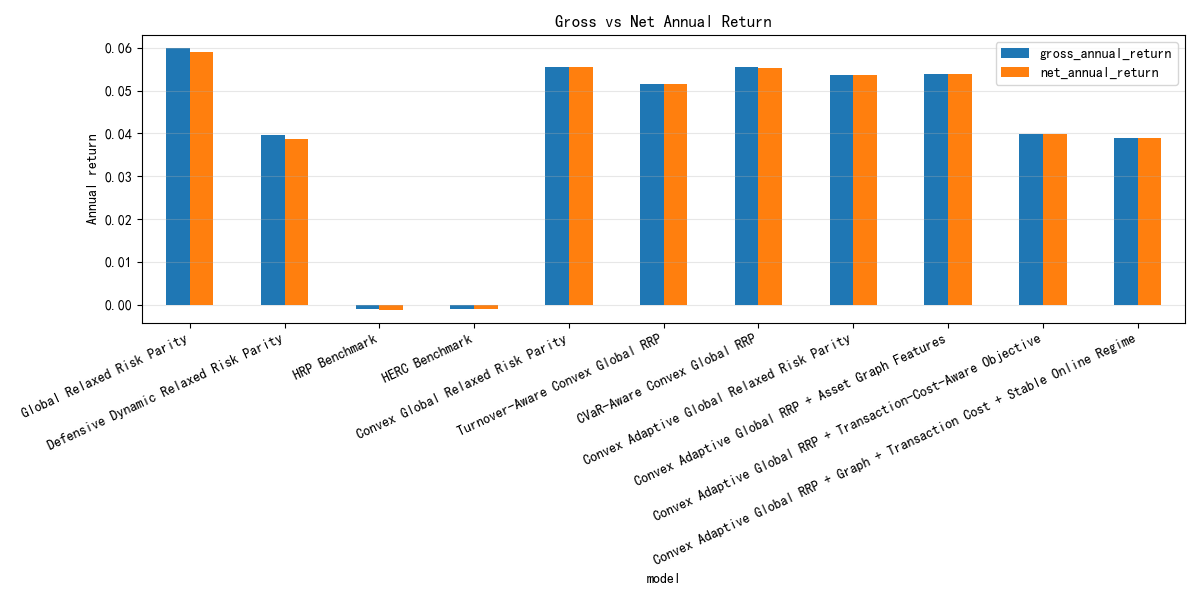
\includegraphics[width=0.88\textwidth,height=0.64\textheight,keepaspectratio]{convex_adaptive_transaction_cost_comparison.png}
  \end{center}
  \vspace{-0.2em}
  \footnotesize\centering
  Global RRP 的年化成本拖累显著高于 Improved Convex；在 \txCostBps{} bps 成本下已不可忽视，若实际成本更高则差距进一步拉大
\end{frame}

\begin{frame}{CVaR 尾部风险对比}
  \begin{center}
    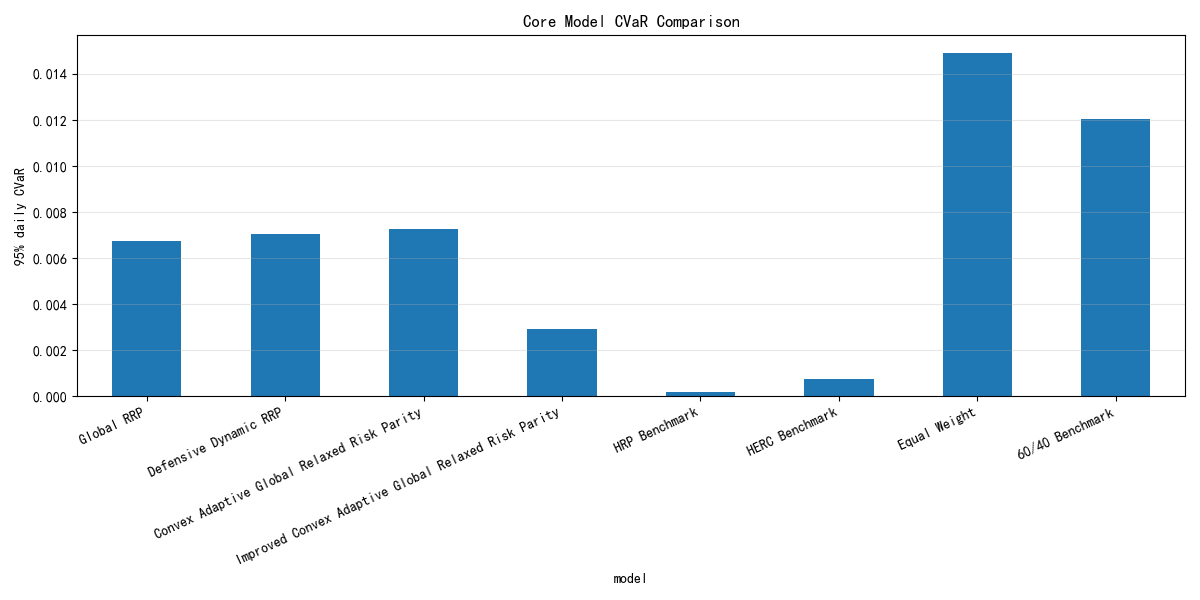
\includegraphics[width=0.88\textwidth,height=0.64\textheight,keepaspectratio]{convex_adaptive_cvar_comparison.png}
  \end{center}
  \vspace{-0.2em}
  \footnotesize\centering
  CVaR 约束在 Improved Convex 中显式限制尾部损失；该约束与 $\ell_1$ 换手惩罚共同作用，是 Sortino 从 \globalSortino{} 升至 \improvedSortino{} 的主要来源
\end{frame}

\begin{frame}{Improved Convex：动态权重路径}
  \begin{center}
    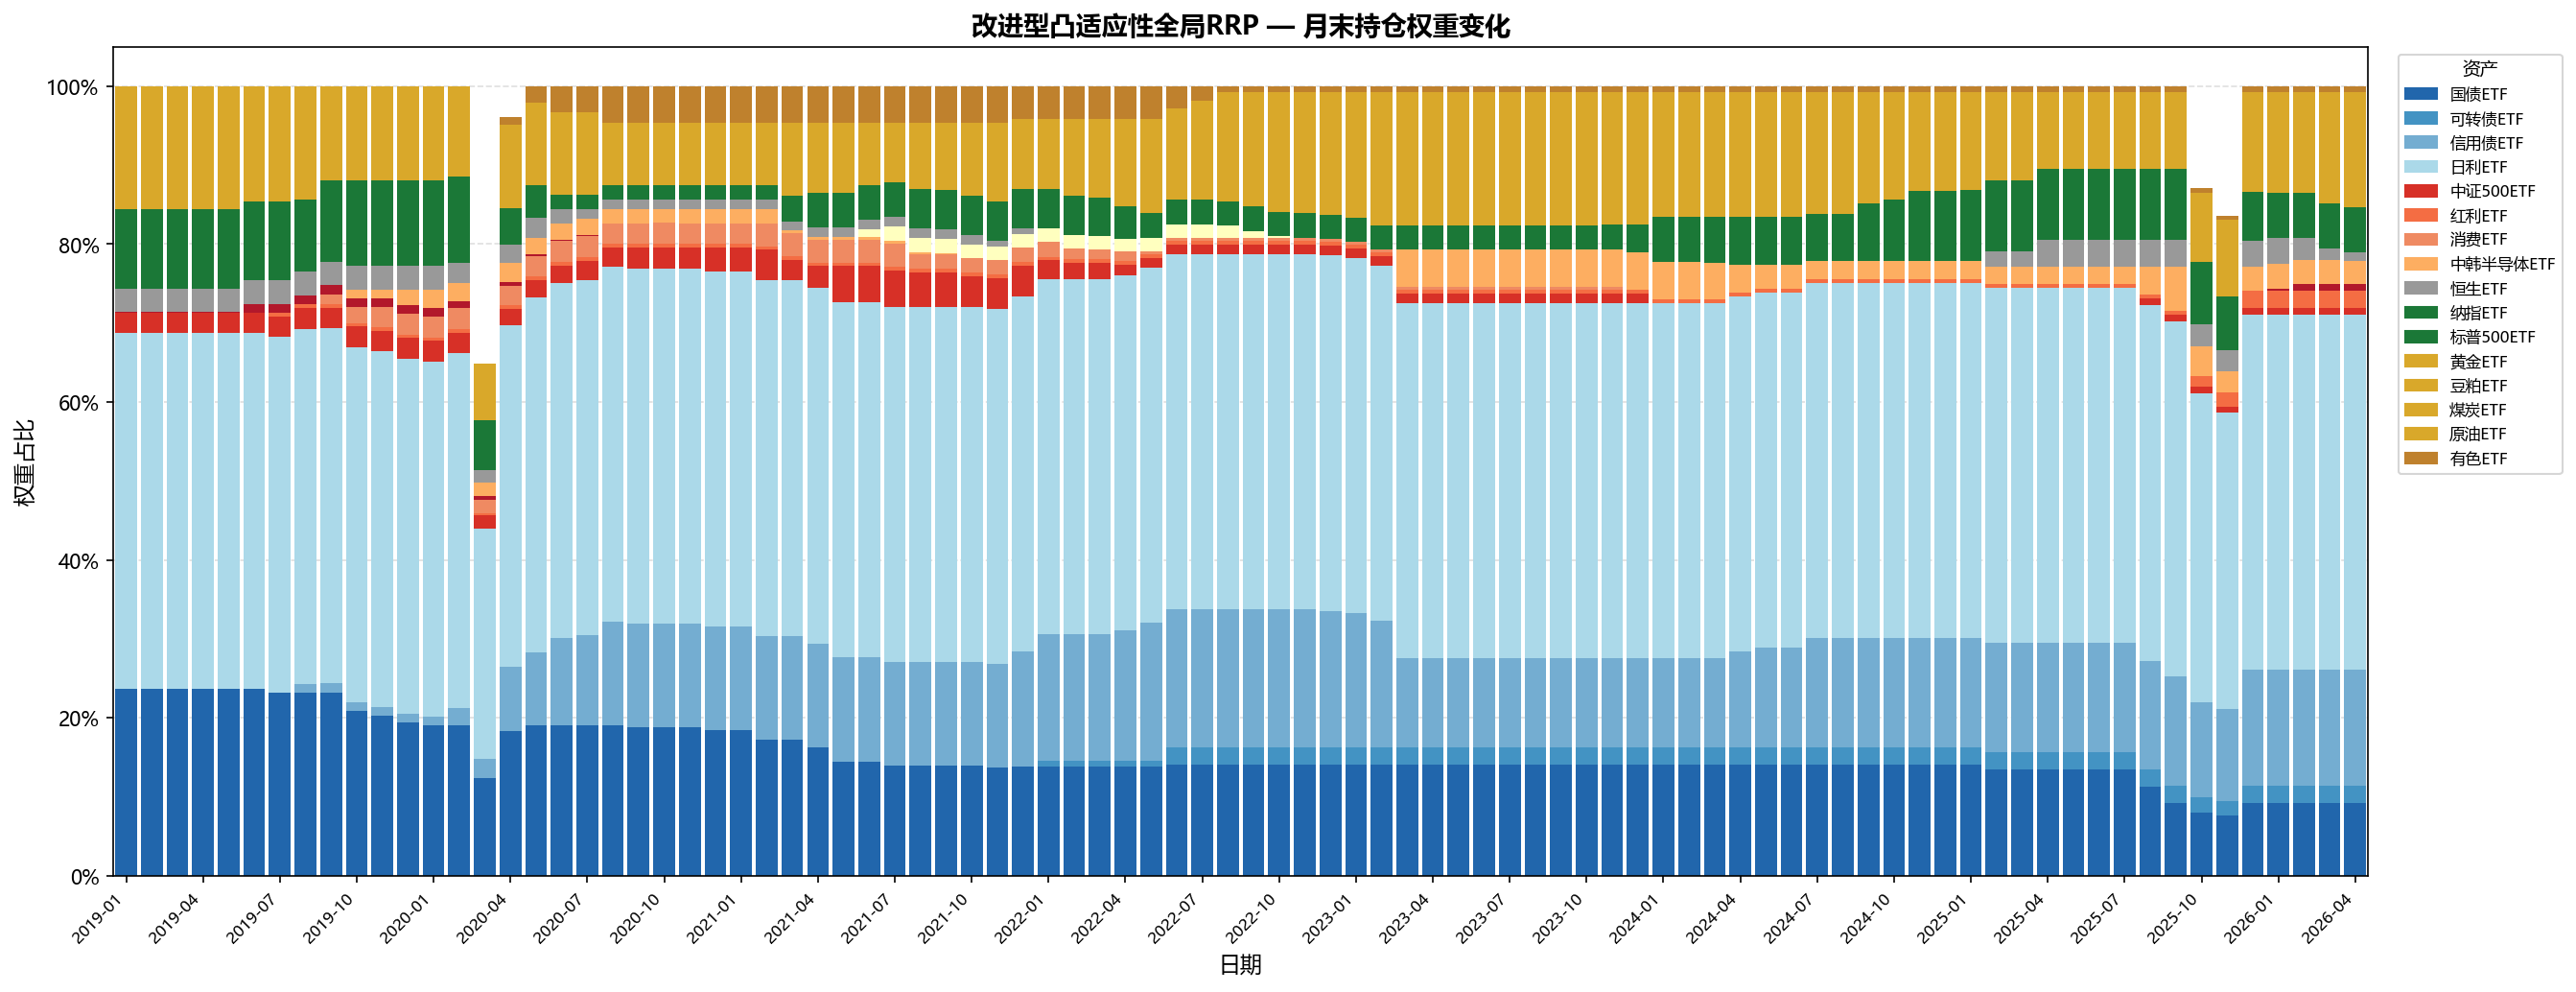
\includegraphics[width=0.88\textwidth,height=0.64\textheight,keepaspectratio]{improved_weights_timeline.png}
  \end{center}
  \vspace{-0.2em}
  \begin{columns}[T]
    \begin{column}{0.50\textwidth}
      \footnotesize
      \begin{itemize}
        \item 换手约束使权重平滑过渡，月度调仓幅度小
      \end{itemize}
    \end{column}
    \begin{column}{0.50\textwidth}
      \footnotesize
      \begin{itemize}
        \item 债券与大宗商品在市场动荡期权重上升，体现防御性
      \end{itemize}
    \end{column}
  \end{columns}
\end{frame}

\begin{frame}{资产组权重路径：各类别占比演变}
  \begin{center}
    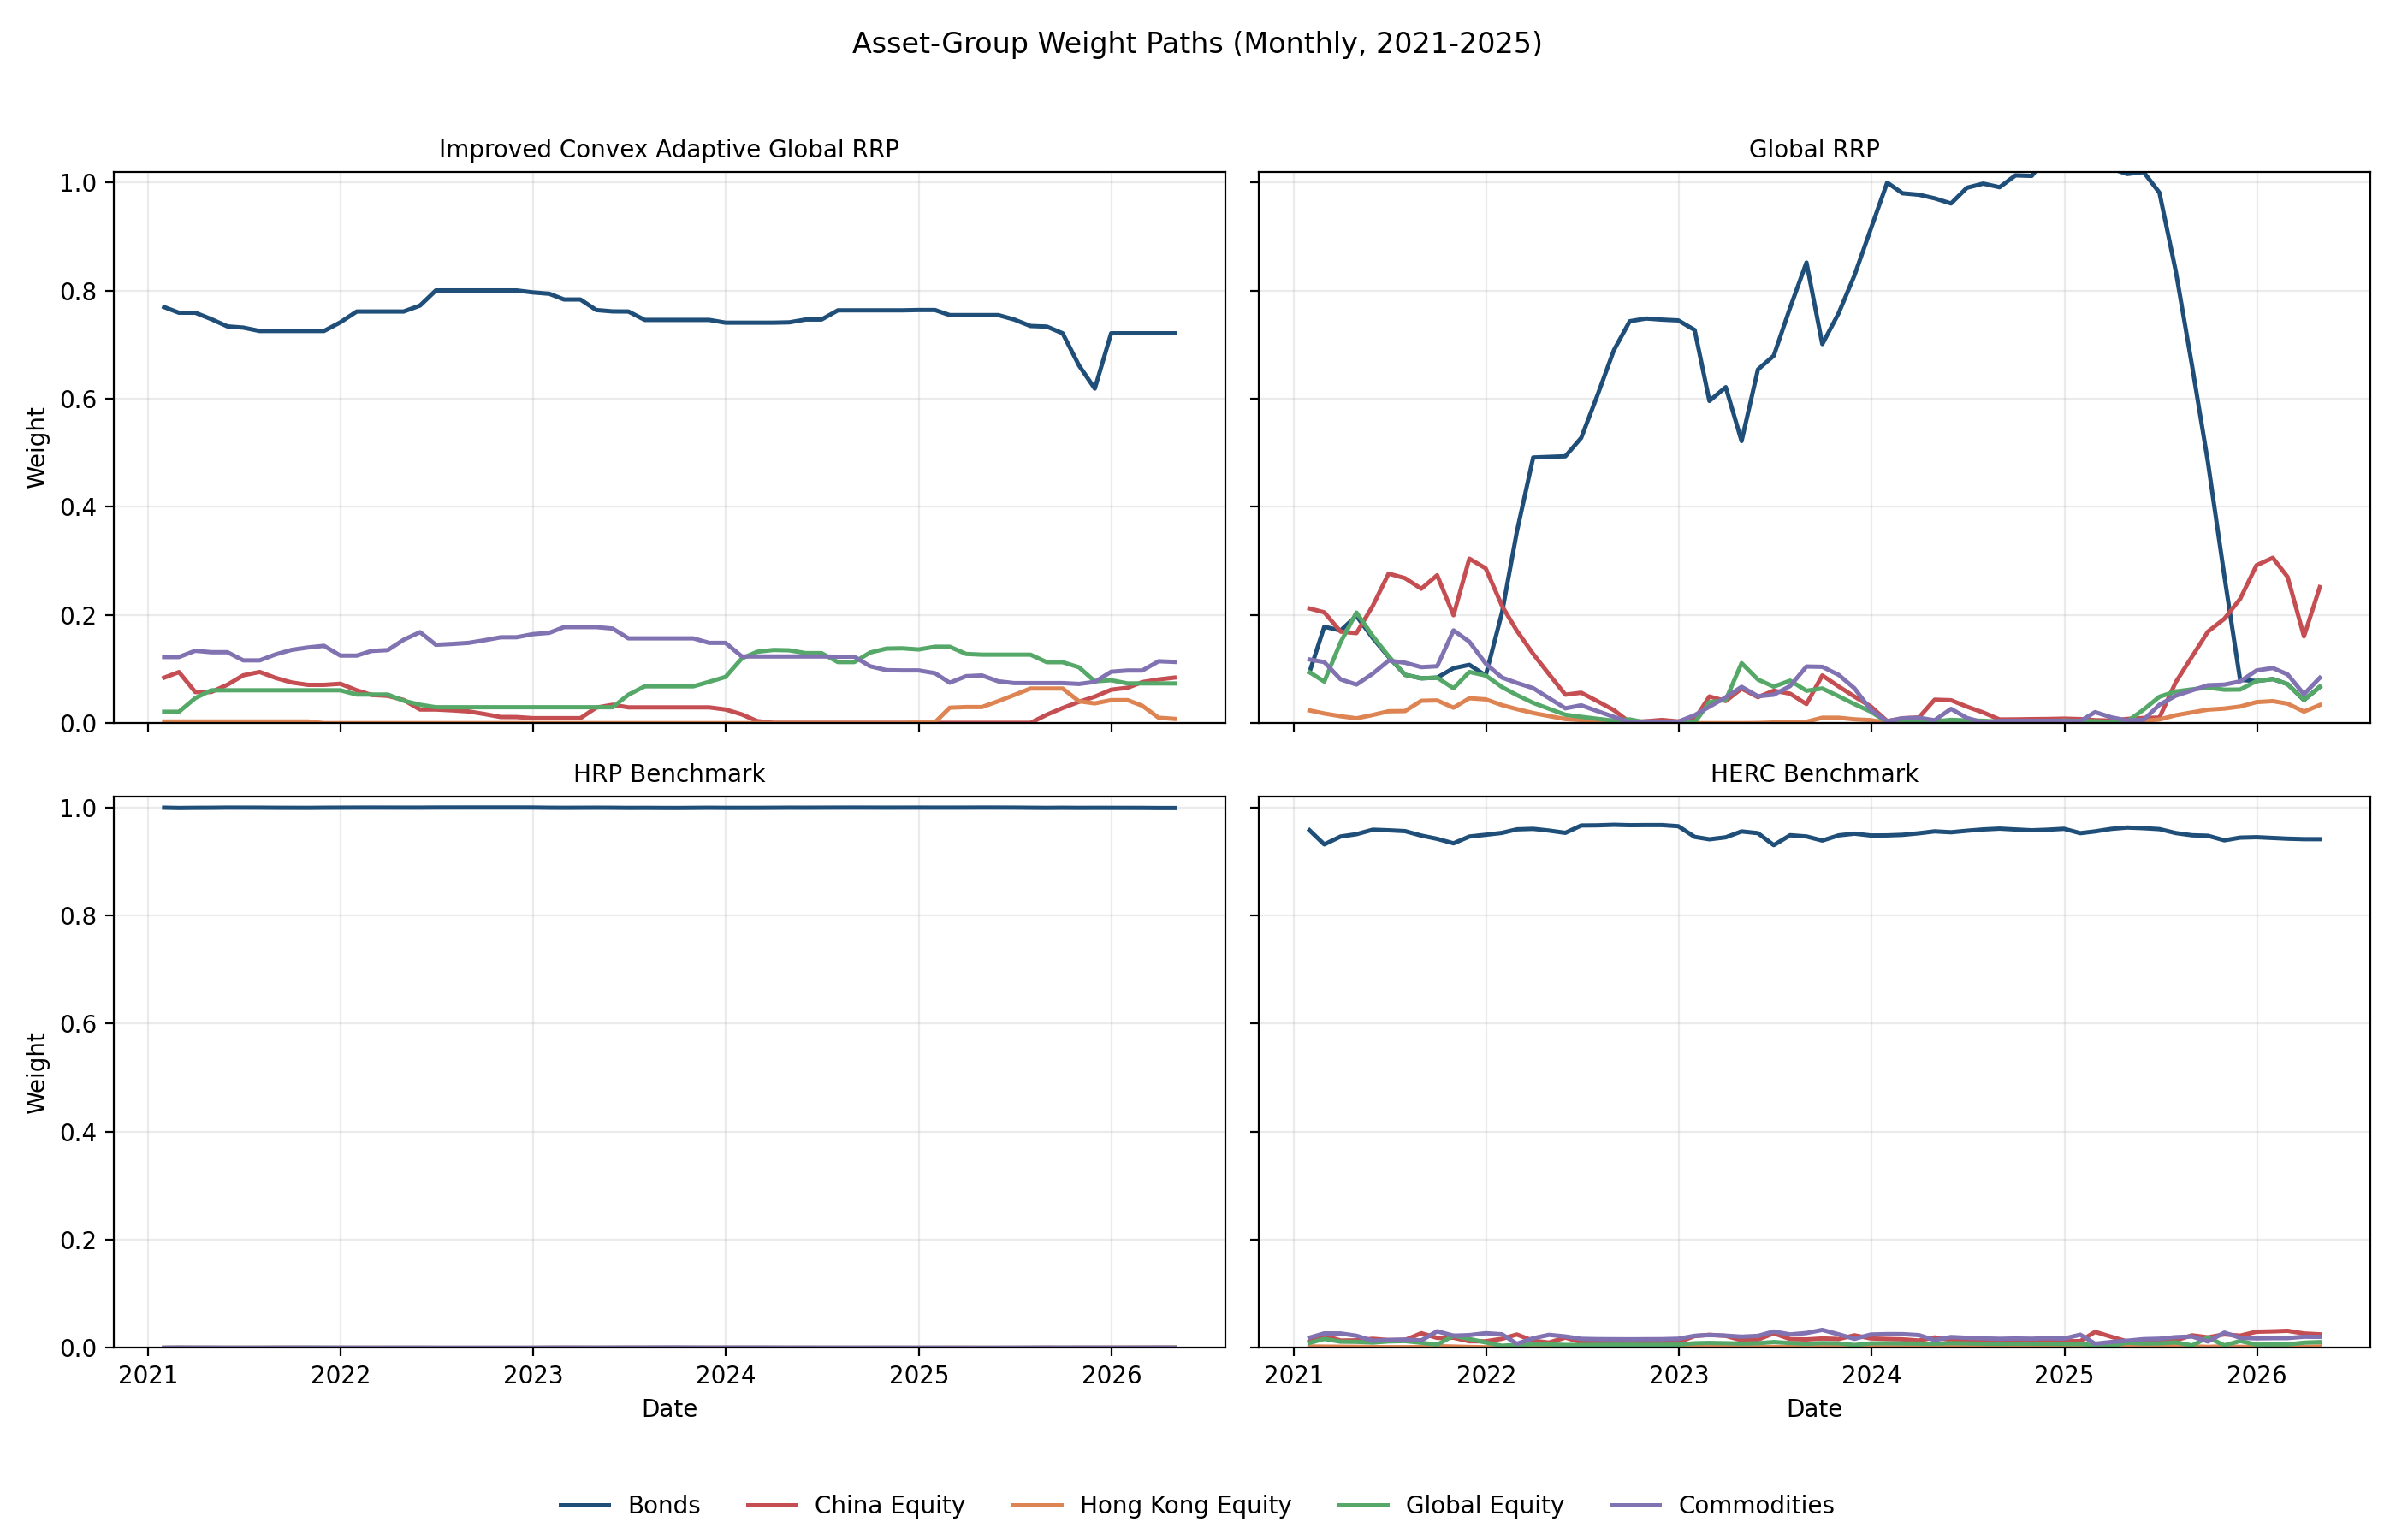
\includegraphics[width=0.88\textwidth,height=0.64\textheight,keepaspectratio]{weight_path_asset_group_comparison.png}
  \end{center}
  \vspace{-0.2em}
  \footnotesize\centering
  各资产组权重在评价期内动态调整，整体保持 8 大类分散，无单一类别长期占比超过组别上限约束
\end{frame}

\begin{frame}{HERC 权重路径：为何 Sharpe 高但无可比性}
  \begin{center}
    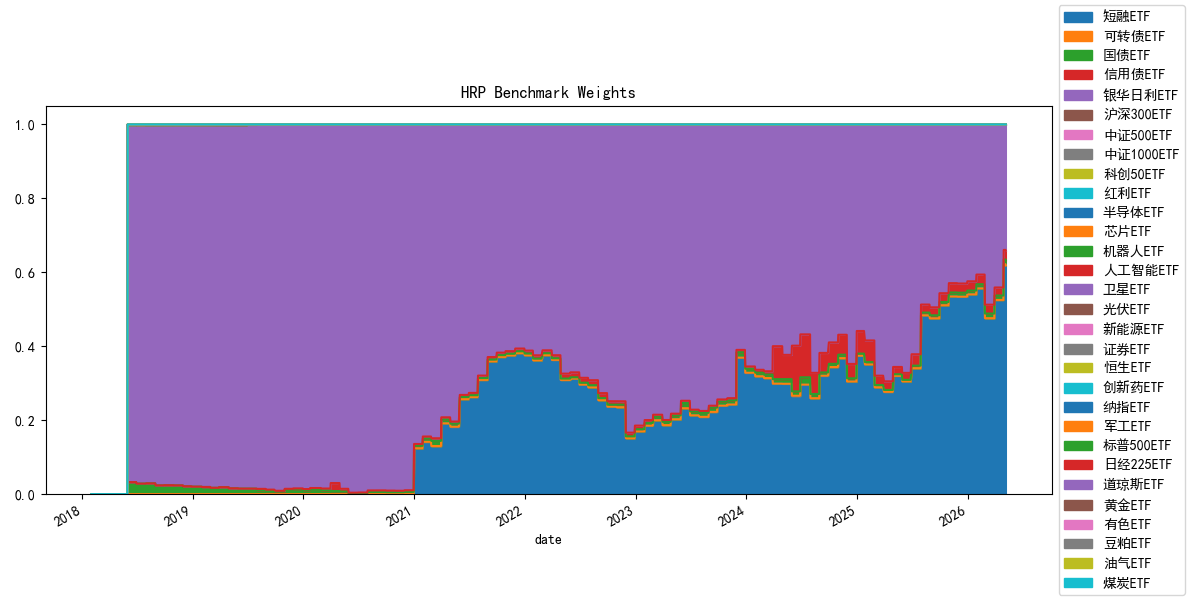
\includegraphics[width=0.88\textwidth,height=0.60\textheight,keepaspectratio]{hrp_weights_timeline.png}
  \end{center}
  \vspace{-0.2em}
  \begin{columns}[T]
    \begin{column}{0.50\textwidth}
      \footnotesize
      \begin{itemize}
        \item HERC 递归二分将几乎全部权重集中于\textbf{日利/国债 ETF}（极低波动）
      \end{itemize}
    \end{column}
    \begin{column}{0.50\textwidth}
      \footnotesize
      \begin{itemize}
        \item 年化波动率 \hercVolatility{}，Sharpe = \hercSharpe{} 来自人工压低分母，而非真正多资产分散
      \end{itemize}
    \end{column}
  \end{columns}
\end{frame}

\begin{frame}{与外部基准对比：净值与回撤}
  \begin{columns}[T]
    \begin{column}{0.50\textwidth}
      \centering
      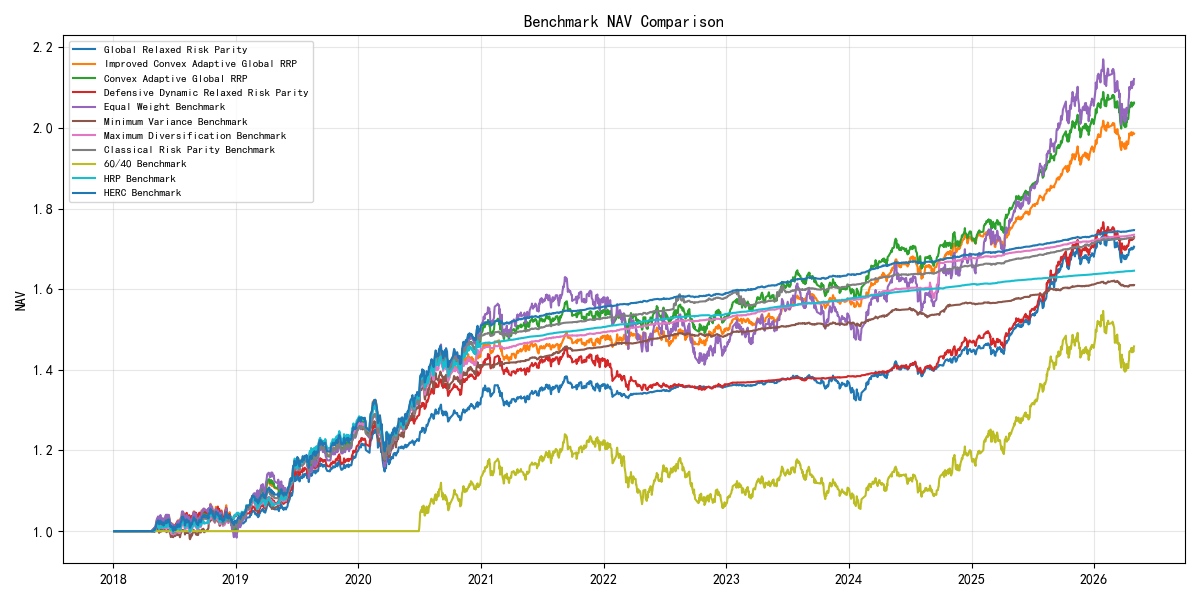
\includegraphics[width=\textwidth,height=0.65\textheight,keepaspectratio]{benchmark_nav_comparison.png}\\
      \footnotesize\centering 净值路径
    \end{column}
    \begin{column}{0.50\textwidth}
      \centering
      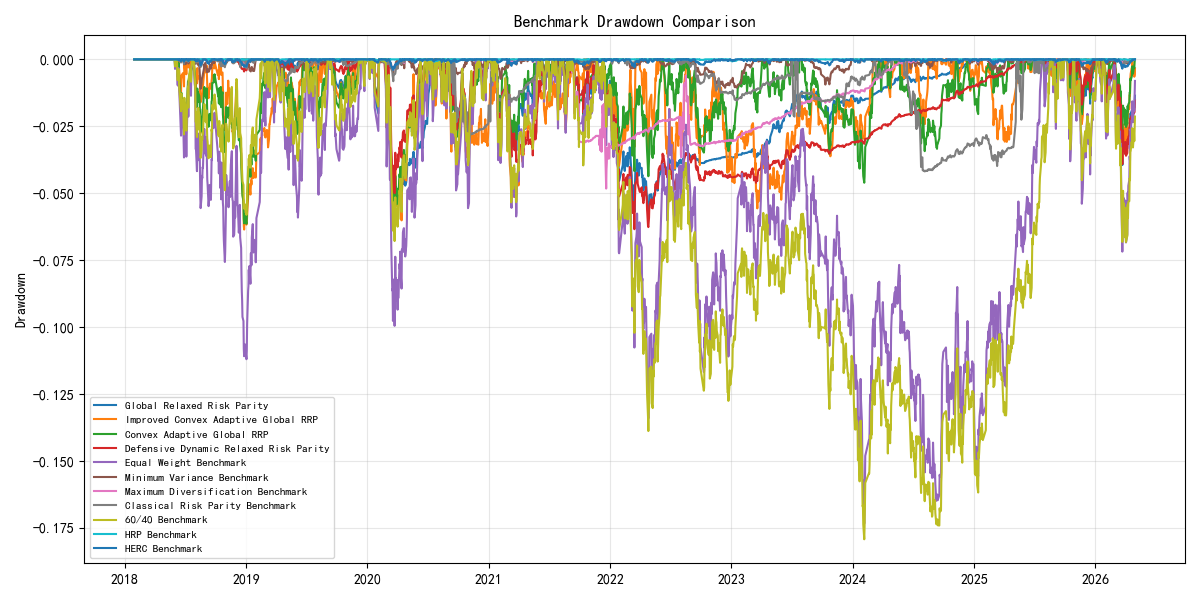
\includegraphics[width=\textwidth,height=0.65\textheight,keepaspectratio]{benchmark_drawdown_comparison.png}\\
      \footnotesize\centering 回撤路径
    \end{column}
  \end{columns}
  \vspace{0.2em}
  \footnotesize\centering
  Improved Convex 净收益 \improvedNetReturn{}，回撤 \improvedMaxDD{}；等权收益更高（\equalNetReturn{}）但回撤 \equalMaxDD{} 为代价；60/40 回撤最深（\sixtyFortyMaxDD{}）
\end{frame}

\begin{frame}{与沪深 300 月度收益散点对比}
  \begin{center}
    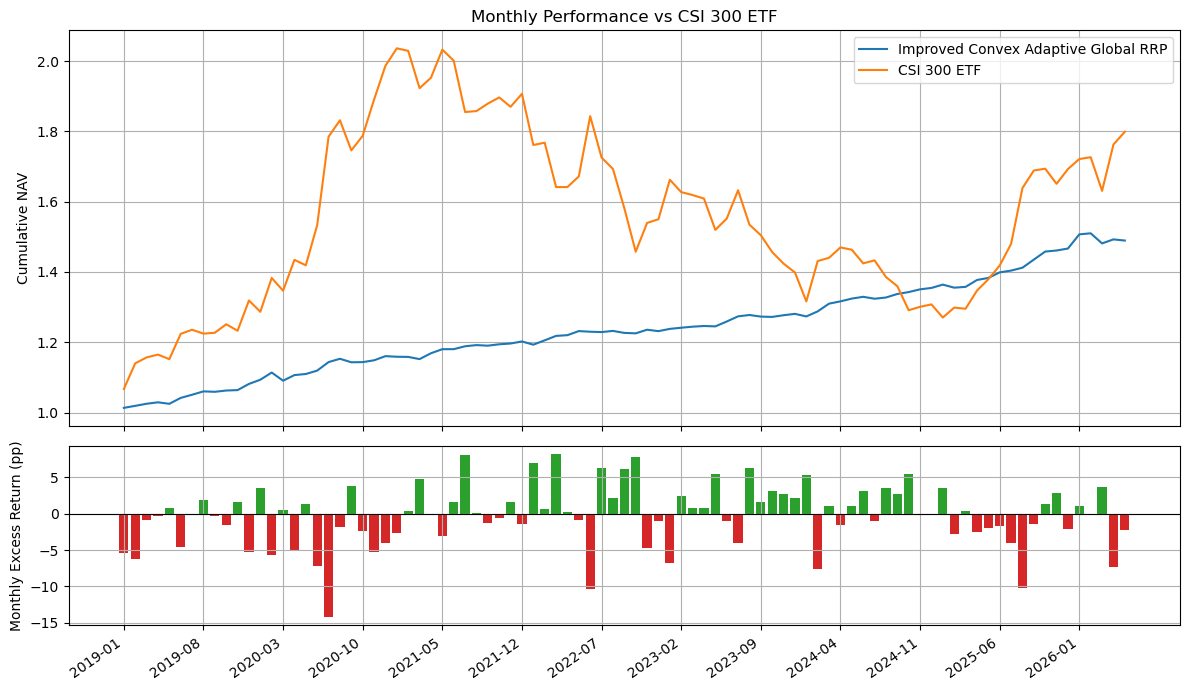
\includegraphics[width=0.88\textwidth,height=0.66\textheight,keepaspectratio]{improved_rrp_vs_hs300_monthly_comparison.png}
  \end{center}
  \vspace{-0.2em}
  \footnotesize\centering
  Improved Convex 对 A 股下行的防御性：沪深 300 大跌月份，组合回撤幅度明显收窄，体现跨资产分散的实际效果
\end{frame}

\begin{frame}{风险归因与收益归因}
  \begin{columns}[T]
    \begin{column}{0.50\textwidth}
      \centering
      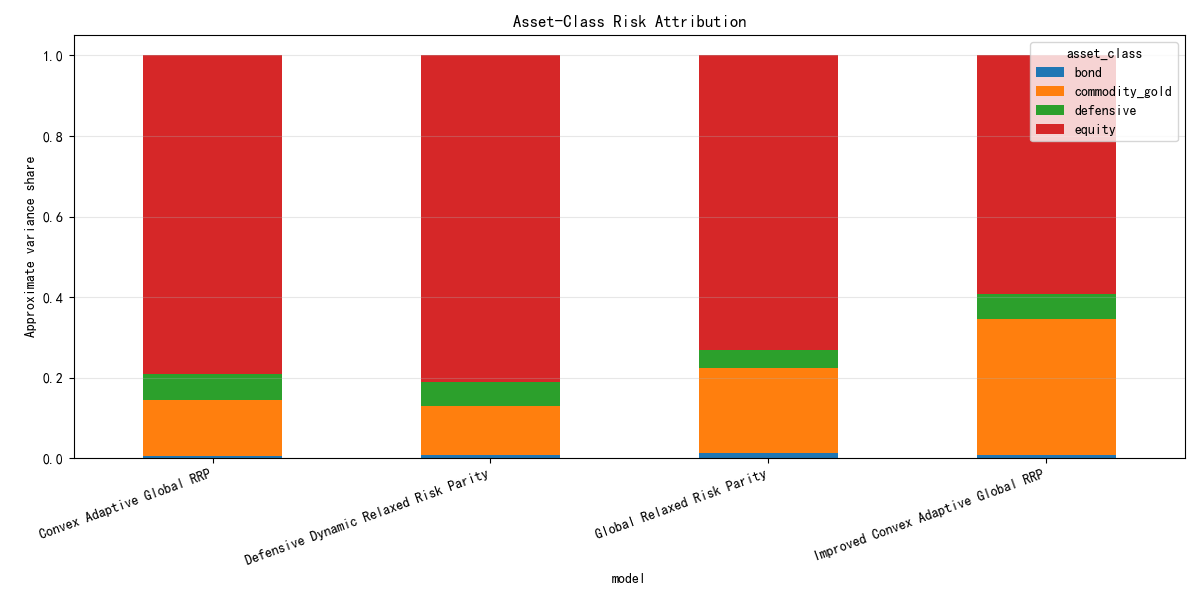
\includegraphics[width=\textwidth,height=0.65\textheight,keepaspectratio]{asset_pricing_risk_attribution.png}\\
      \footnotesize\centering 风险归因（各资产对组合波动的贡献）
    \end{column}
    \begin{column}{0.50\textwidth}
      \centering
      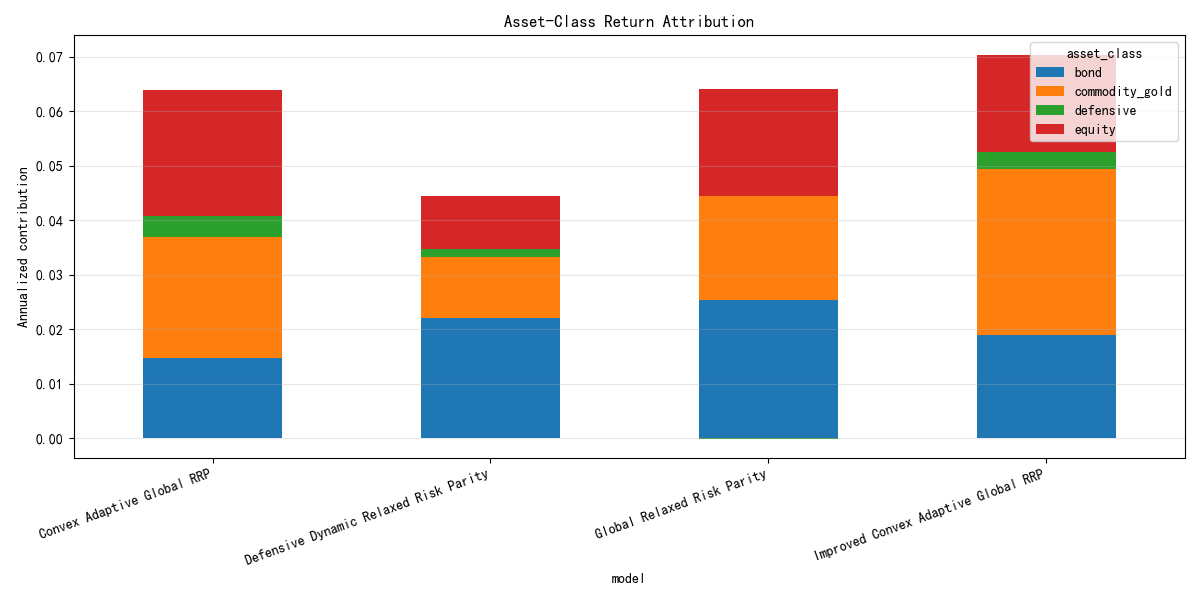
\includegraphics[width=\textwidth,height=0.65\textheight,keepaspectratio]{asset_pricing_return_attribution.png}\\
      \footnotesize\centering 收益归因（各资产对累计净值的贡献）
    \end{column}
  \end{columns}
  \vspace{0.2em}
  \footnotesize\centering
  债券类贡献大部分风险预算（符合风险平价设计）；大宗商品和科技 ETF 提供超额收益来源
\end{frame}

\begin{frame}{滚动因子 Beta：风格暴露动态变化}
  \begin{center}
    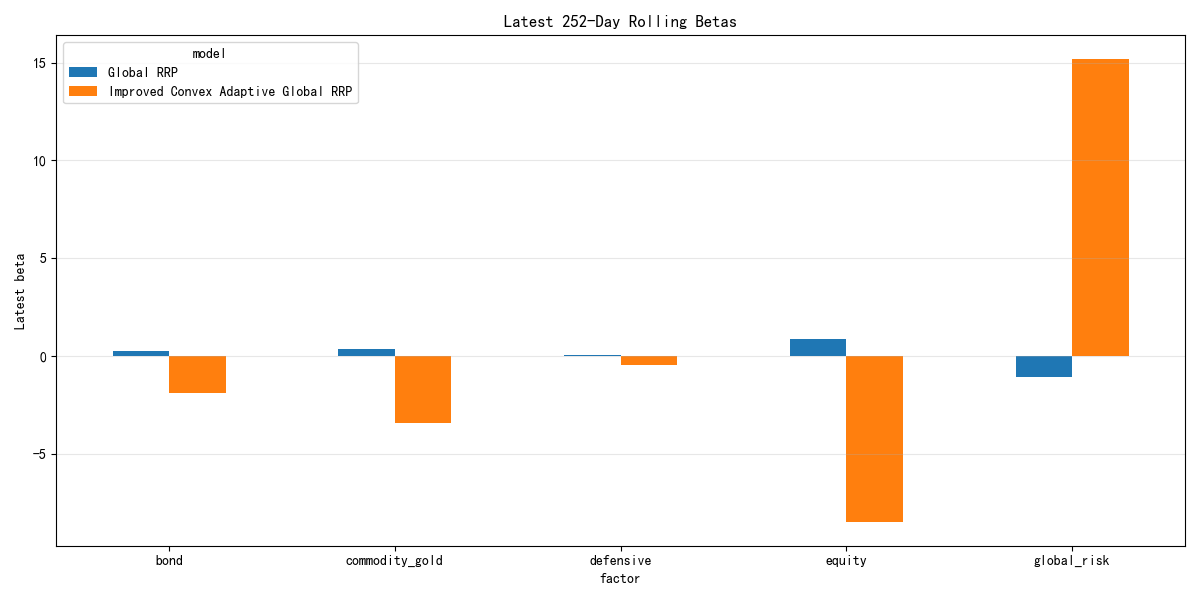
\includegraphics[width=0.88\textwidth,height=0.66\textheight,keepaspectratio]{asset_pricing_rolling_betas.png}
  \end{center}
  \vspace{-0.2em}
  \footnotesize\centering
  组合对各风险因子的敞口随市场环境动态调整，整体保持分散而非单一因子押注
\end{frame}

\begin{frame}{参数动态时序：$\lambda$ 选择的演变}
  \begin{center}
    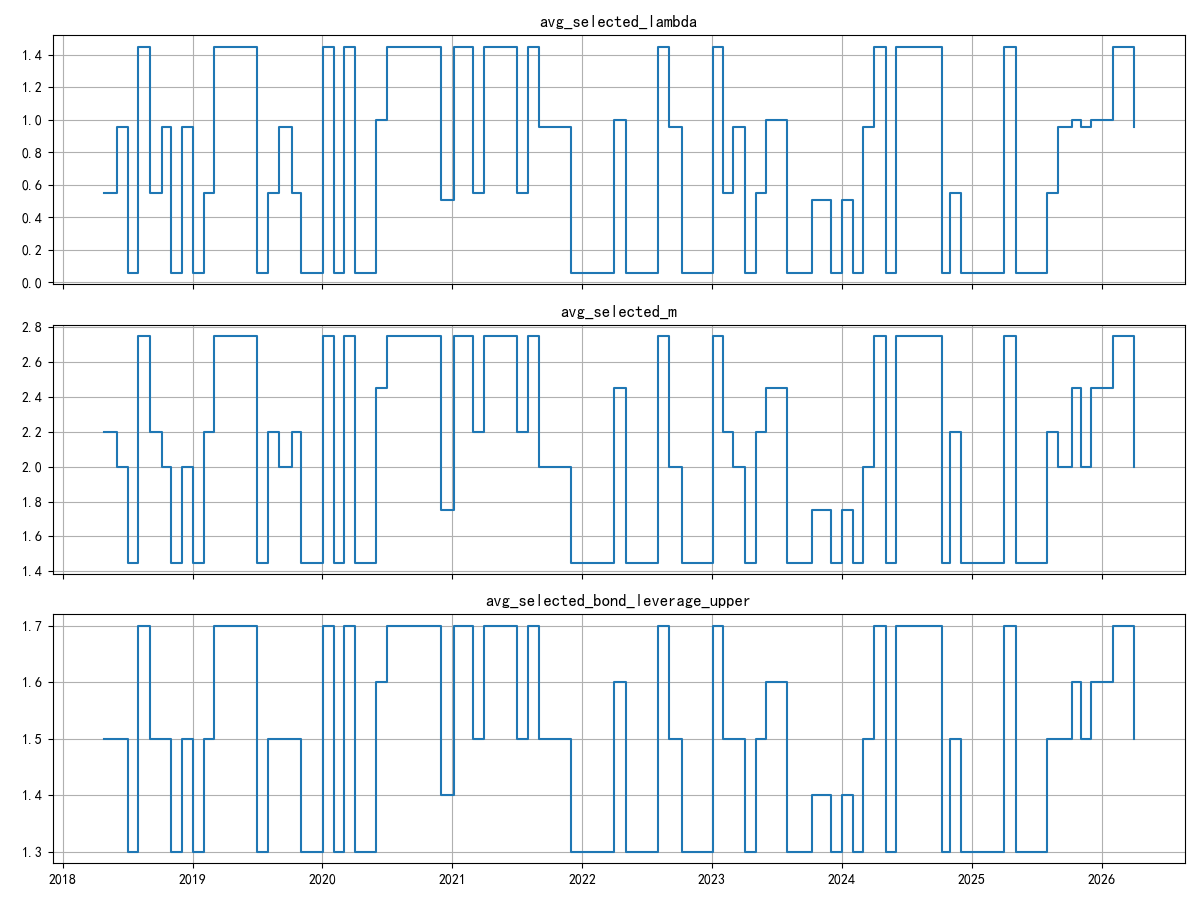
\includegraphics[width=0.88\textwidth,height=0.66\textheight,keepaspectratio]{showcase_parameter_timeline.png}
  \end{center}
  \vspace{-0.2em}
  \footnotesize\centering
  各惩罚系数在样本期内的时序变化；冻结参数后所有系数固定不变，图示用于诊断候选参数的历史行为
\end{frame}

\begin{frame}{风险覆盖层消融实验}
  \begin{center}
    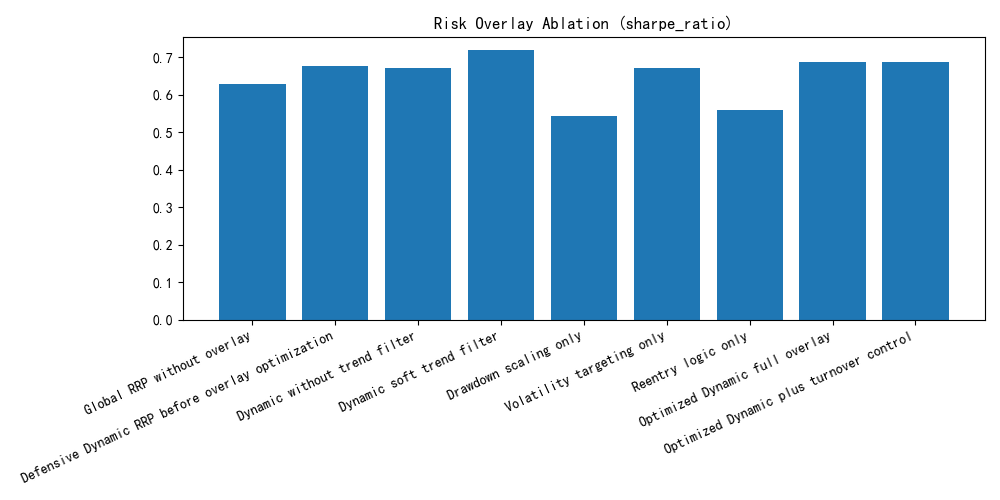
\includegraphics[width=0.88\textwidth,height=0.62\textheight,keepaspectratio]{showcase_risk_overlay_ablation.png}
  \end{center}
  \vspace{-0.2em}
  \begin{columns}[T]
    \begin{column}{0.50\textwidth}
      \footnotesize
      \begin{itemize}
        \item 逐步剥离 CVaR 约束、换手惩罚、资产组上限，观察各约束的\textbf{独立贡献}
      \end{itemize}
    \end{column}
    \begin{column}{0.50\textwidth}
      \footnotesize
      \begin{itemize}
        \item 移除 CVaR 约束后尾部损失显著扩大；移除换手惩罚后成本拖累回升
      \end{itemize}
    \end{column}
  \end{columns}
\end{frame}

\begin{frame}{Sharpe 差异统计检验}
  \begin{columns}[T]
    \begin{column}{0.60\textwidth}
      \footnotesize\renewcommand{\arraystretch}{1.35}
      \begin{tabular}{@{}lccc@{}}
        \toprule
        比较对 & $\Delta$Sharpe & $p$ 值 & 结论 \\
        \midrule
        Improved vs.\ Global RRP & \improvedVsGlobalDiff & \improvedVsGlobalPValue & \textbf{显著} \\
        Improved vs.\ Defensive  & 0.893 & 0.001 & \textbf{显著} \\
        Improved vs.\ 等权       & 0.686 & 0.013 & \textbf{显著} \\
        Global vs.\ 等权         & $-$0.071 & 0.782 & 不显著 \\
        Defensive vs.\ 等权      & $-$0.185 & 0.434 & 不显著 \\
        \bottomrule
      \end{tabular}
      \vspace{0.3em}
      \scriptsize 基于 Jobson-Korkie 检验，Bootstrap 95\% 置信区间
    \end{column}
    \begin{column}{0.37\textwidth}
      \begin{block}{核心含义}
        \footnotesize
        \begin{itemize}
          \item Improved Convex 优势\textbf{统计显著}（$p=\improvedVsGlobalPValue$）
          \item 仅降换手不足以产生显著 Sharpe 提升
          \item \textbf{CVaR + 参数冻结}是真实来源
        \end{itemize}
      \end{block}
    \end{column}
  \end{columns}
\end{frame}

% ════════════════════════════════════════════════════════════════════════════
\section{稳健性检验}
% ════════════════════════════════════════════════════════════════════════════

\begin{frame}{稳健性检验体系：五个维度}
  \begin{columns}[T]
    \begin{column}{0.50\textwidth}
      \begin{enumerate}
        \item \textbf{Walk-forward 子区间}：滚动训练-测试窗口，检验跨期稳定性
        \item \textbf{参数扰动}：对 5 个超参数各自 ±20\% 扰动，观察 Sharpe 和换手的分布范围
        \item \textbf{交易成本敏感性}：从 0 到 50+ bps 扫描，确定盈亏平衡阈值
      \end{enumerate}
    \end{column}
    \begin{column}{0.47\textwidth}
      \begin{enumerate}\setcounter{enumi}{3}
        \item \textbf{Bootstrap 分布}：对月度收益序列重抽样，获取 Sharpe 和最大回撤的经验分布
        \item \textbf{协方差估计器}：比较样本协方差、EWMA（基准）、收缩估计三种方案
      \end{enumerate}
      \vspace{0.4em}
      \begin{alertblock}{目标}
        \small 将结论\textbf{明确限定}在特定样本区间和参数设定，避免过度外推
      \end{alertblock}
    \end{column}
  \end{columns}
\end{frame}

\begin{frame}{Walk-forward：子区间 Sharpe 与最大回撤}
  \begin{columns}[T]
    \begin{column}{0.50\textwidth}
      \centering
      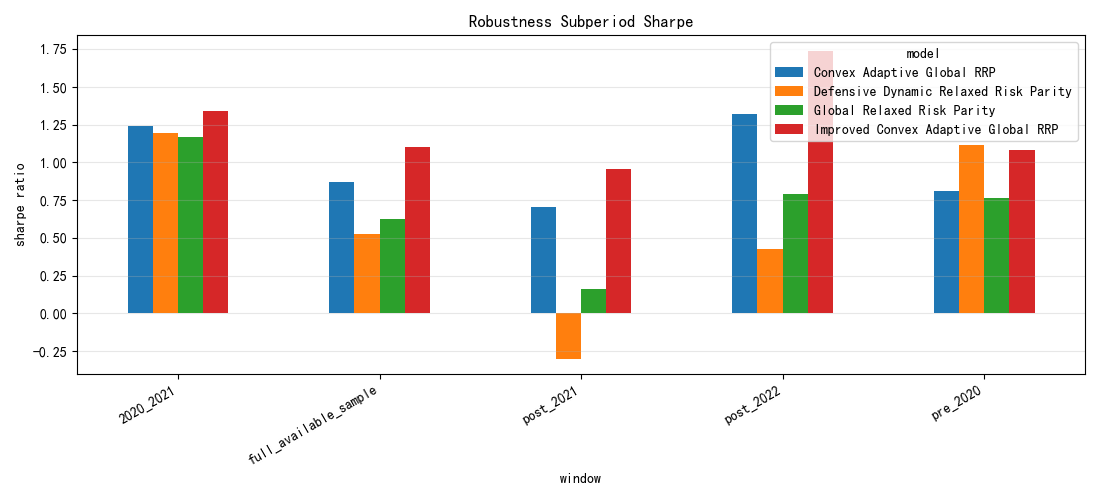
\includegraphics[width=\textwidth,height=0.64\textheight,keepaspectratio]{robustness_subperiod_sharpe.png}\\
      \footnotesize\centering Sharpe 比率（中位数 \wfSharpeMedian{}，均值 \wfSharpeMean{}）
    \end{column}
    \begin{column}{0.50\textwidth}
      \centering
      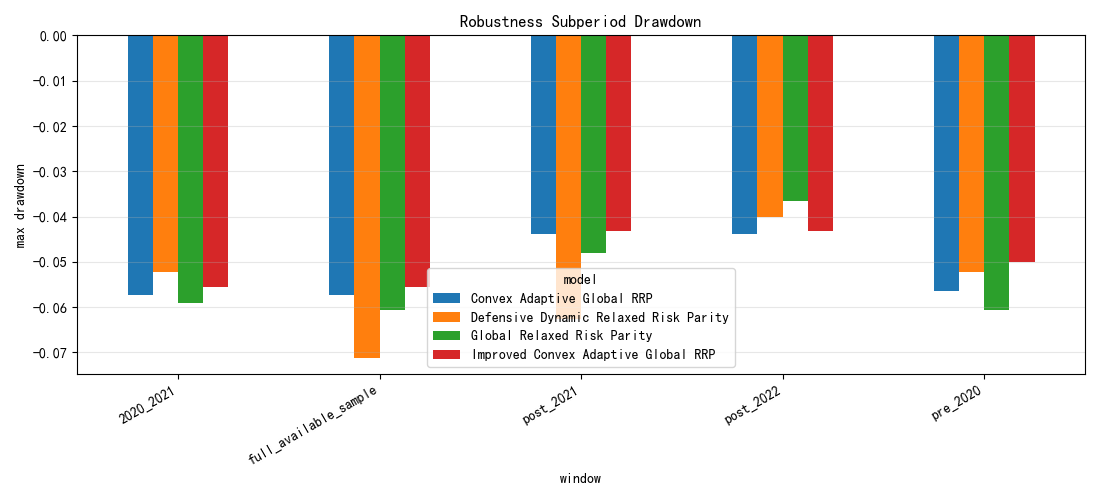
\includegraphics[width=\textwidth,height=0.64\textheight,keepaspectratio]{robustness_subperiod_drawdown.png}\\
      \footnotesize\centering 最大回撤（均值 \wfDDMean{}）
    \end{column}
  \end{columns}
  \vspace{0.2em}
  \footnotesize\centering
  多数子区间 Sharpe $>$ 0.8，中位数约 1.0；加息冲击期（2022）表现最弱，但未出现大幅回撤
\end{frame}

\begin{frame}{参数扰动敏感性分析}
  \begin{center}
    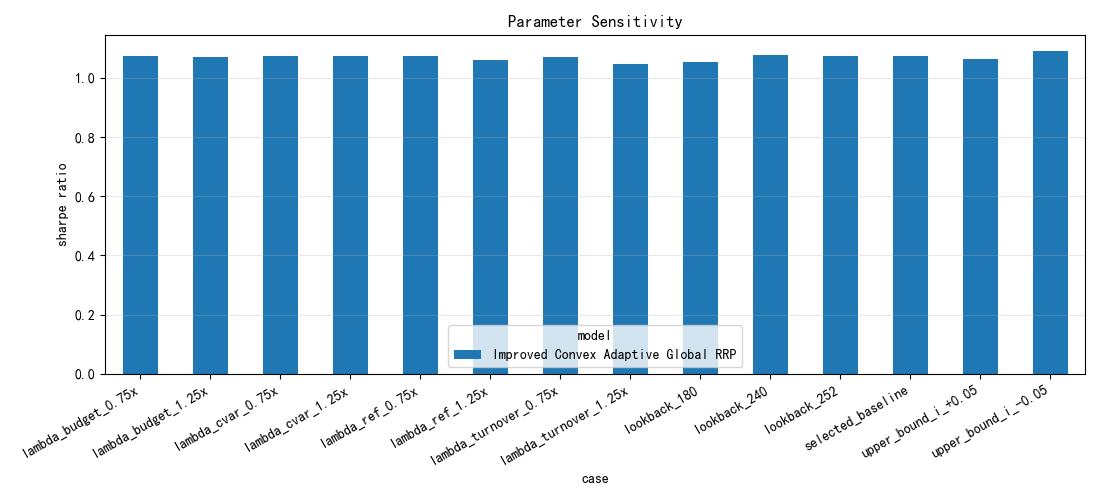
\includegraphics[width=0.88\textwidth,height=0.64\textheight,keepaspectratio]{robustness_parameter_sensitivity.png}
  \end{center}
  \vspace{-0.2em}
  \begin{columns}[T]
    \begin{column}{0.50\textwidth}
      \footnotesize
      \begin{itemize}
        \item Sharpe 对换手惩罚系数 $\lambda_{to}$ 最敏感——说明换手控制是关键杠杆
      \end{itemize}
    \end{column}
    \begin{column}{0.50\textwidth}
      \footnotesize
      \begin{itemize}
        \item CVaR 系数 $\lambda_c$ 扰动对最大回撤影响显著，整体方向稳定
      \end{itemize}
    \end{column}
  \end{columns}
\end{frame}

\begin{frame}{交易成本敏感性：盈亏平衡分析}
  \begin{center}
    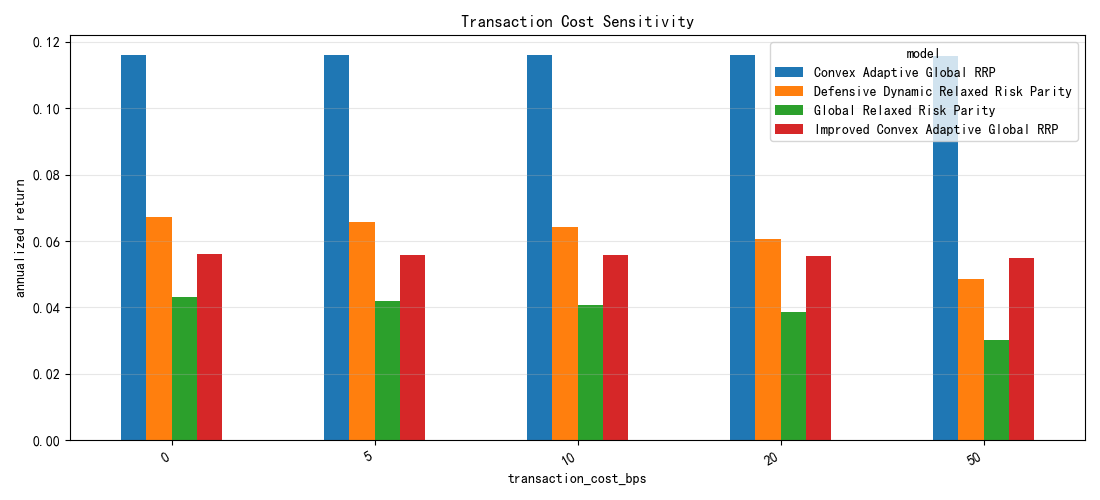
\includegraphics[width=0.88\textwidth,height=0.64\textheight,keepaspectratio]{robustness_transaction_cost_sensitivity.png}
  \end{center}
  \vspace{-0.2em}
  \begin{columns}[T]
    \begin{column}{0.50\textwidth}
      \footnotesize
      \begin{itemize}
        \item Improved vs.\ Global RRP 的盈亏平衡成本 \textbf{$>$50 bps}，实际 \txCostBps{} bps 远低于此
      \end{itemize}
    \end{column}
    \begin{column}{0.50\textwidth}
      \footnotesize
      \begin{itemize}
        \item 换手率越低的模型，盈亏平衡点越高，对成本假设越不敏感
      \end{itemize}
    \end{column}
  \end{columns}
\end{frame}

\begin{frame}{Bootstrap 经验分布：Sharpe 与最大回撤}
  \begin{columns}[T]
    \begin{column}{0.50\textwidth}
      \centering
      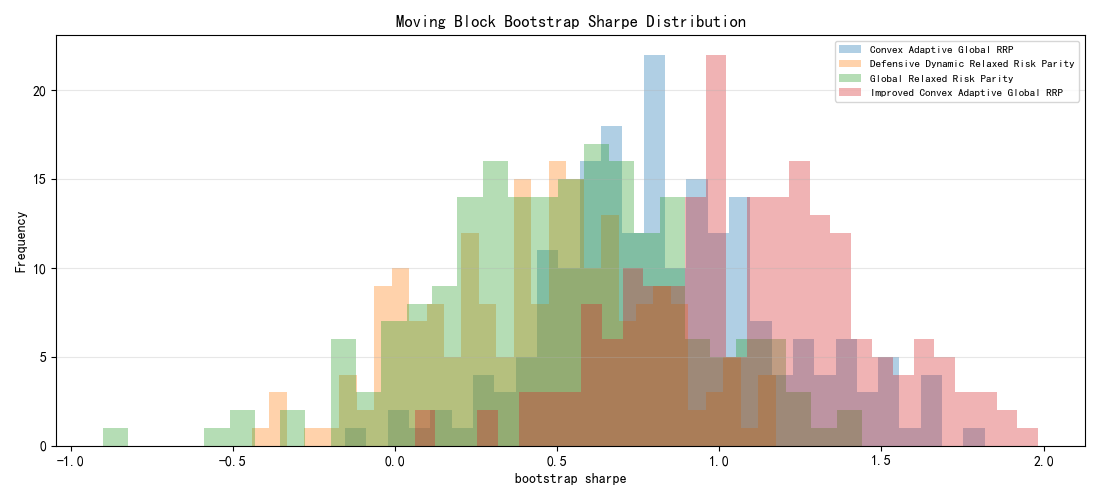
\includegraphics[width=\textwidth,height=0.64\textheight,keepaspectratio]{robustness_bootstrap_sharpe_distribution.png}\\
      \footnotesize\centering Sharpe 经验分布
    \end{column}
    \begin{column}{0.50\textwidth}
      \centering
      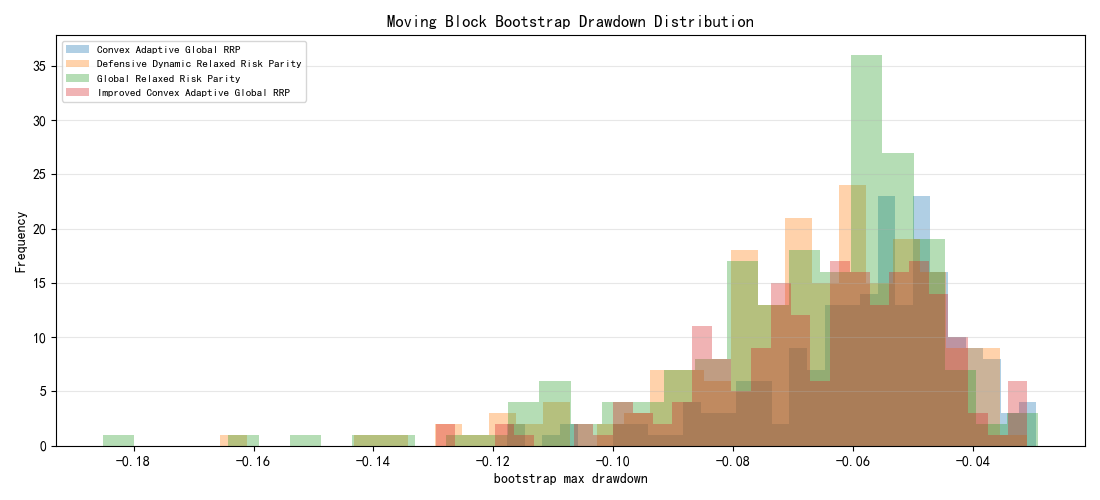
\includegraphics[width=\textwidth,height=0.64\textheight,keepaspectratio]{robustness_bootstrap_drawdown_distribution.png}\\
      \footnotesize\centering 最大回撤经验分布
    \end{column}
  \end{columns}
  \vspace{0.2em}
  \footnotesize\centering
  Bootstrap 1000 次重抽样；Improved Convex 的 Sharpe 分布中心高于其他模型，分布尾部亦较轻
\end{frame}

\begin{frame}{过拟合诊断}
  \begin{center}
    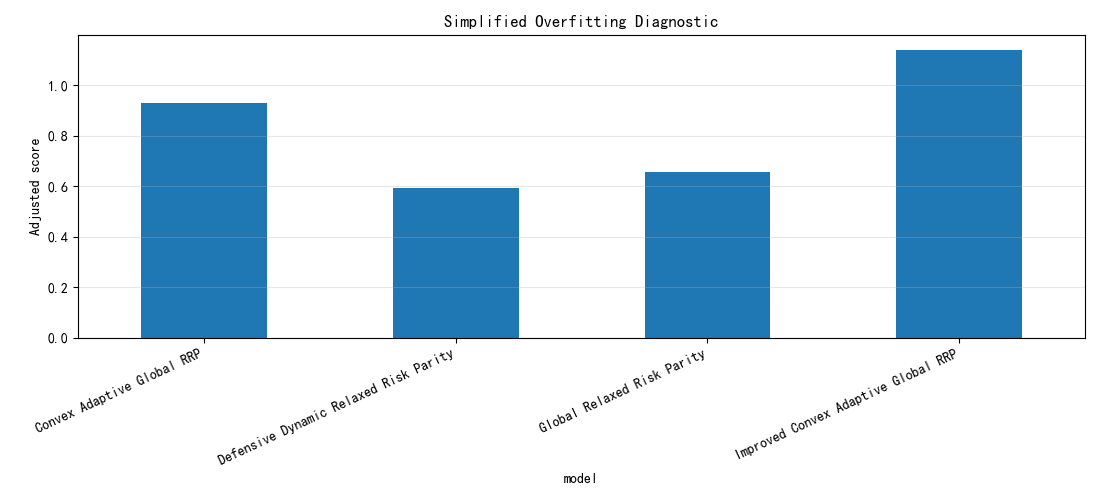
\includegraphics[width=0.88\textwidth,height=0.64\textheight,keepaspectratio]{robustness_overfitting_diagnostic.png}
  \end{center}
  \vspace{-0.2em}
  \begin{columns}[T]
    \begin{column}{0.50\textwidth}
      \footnotesize
      \begin{itemize}
        \item 训练期与 OOS 期绩效差距在可接受范围内，未见明显过拟合迹象
      \end{itemize}
    \end{column}
    \begin{column}{0.50\textwidth}
      \footnotesize
      \begin{itemize}
        \item 参数冻结策略（不在 OOS 期重新优化）是保持诊断结果干净的关键
      \end{itemize}
    \end{column}
  \end{columns}
\end{frame}

\begin{frame}{PBO 热图：概率回测过拟合}
  \begin{center}
    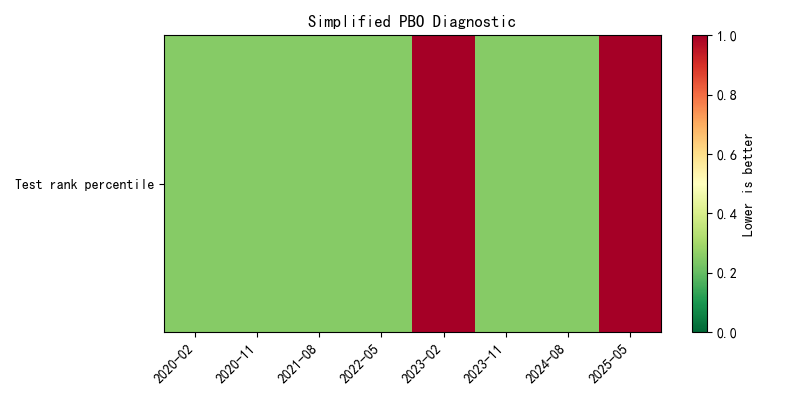
\includegraphics[width=0.88\textwidth,height=0.66\textheight,keepaspectratio]{showcase_pbo_heatmap.png}
  \end{center}
  \vspace{-0.2em}
  \footnotesize\centering
  PBO（Probability of Backtest Overfitting）热图展示不同超参数组合的过拟合概率；所选参数（candidate\_23）处于低 PBO 区域
\end{frame}

\begin{frame}{协方差估计器对比：Sharpe 与换手}
  \begin{columns}[T]
    \begin{column}{0.50\textwidth}
      \centering
      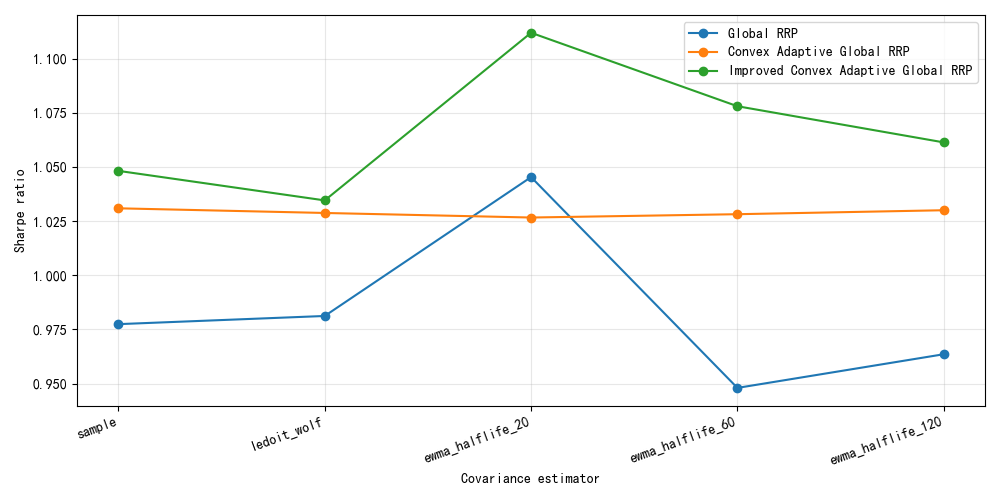
\includegraphics[width=\textwidth,height=0.64\textheight,keepaspectratio]{covariance_robustness_sharpe.png}\\
      \footnotesize\centering Sharpe 比率对比
    \end{column}
    \begin{column}{0.50\textwidth}
      \centering
      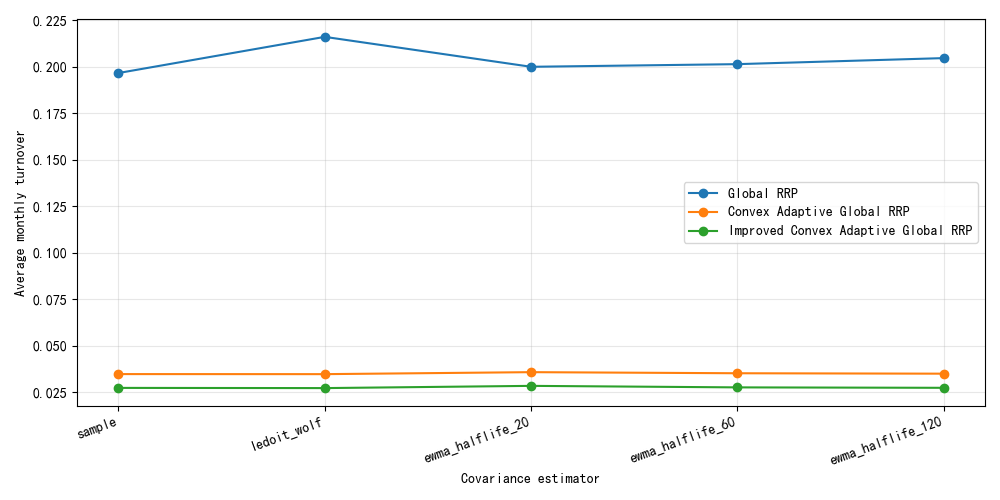
\includegraphics[width=\textwidth,height=0.64\textheight,keepaspectratio]{covariance_robustness_turnover.png}\\
      \footnotesize\centering 换手率对比
    \end{column}
  \end{columns}
  \vspace{0.2em}
  \footnotesize\centering
  样本协方差、EWMA（基准）、收缩估计三种方案下，结论方向一致；EWMA 在换手稳定性上最优
\end{frame}

\begin{frame}{压力期表现：市场动荡时的防御性}
  \begin{columns}[T]
    \begin{column}{0.50\textwidth}
      \centering
      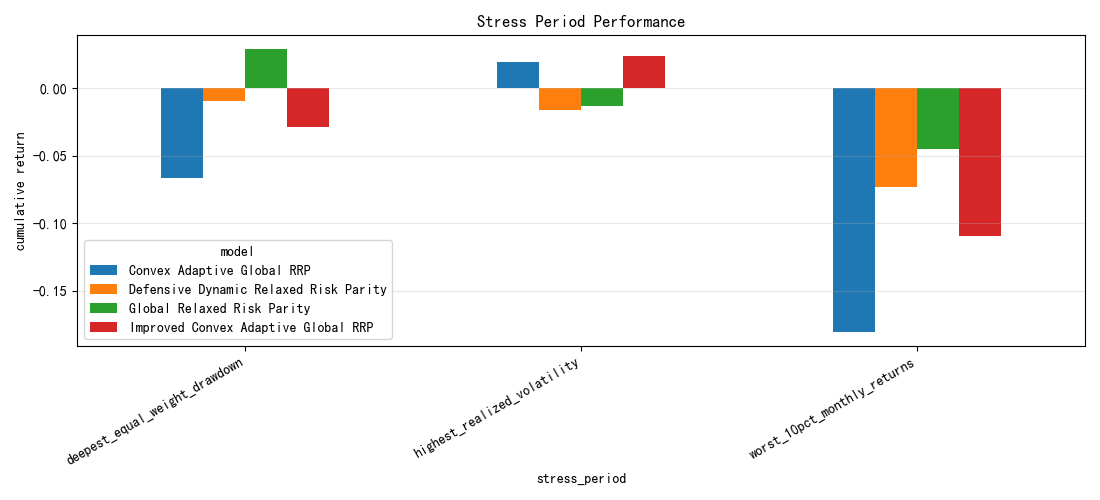
\includegraphics[width=\textwidth,height=0.65\textheight,keepaspectratio]{robustness_stress_period_performance.png}\\
      \footnotesize\centering 各压力期分模型绩效
    \end{column}
    \begin{column}{0.50\textwidth}
      \centering
      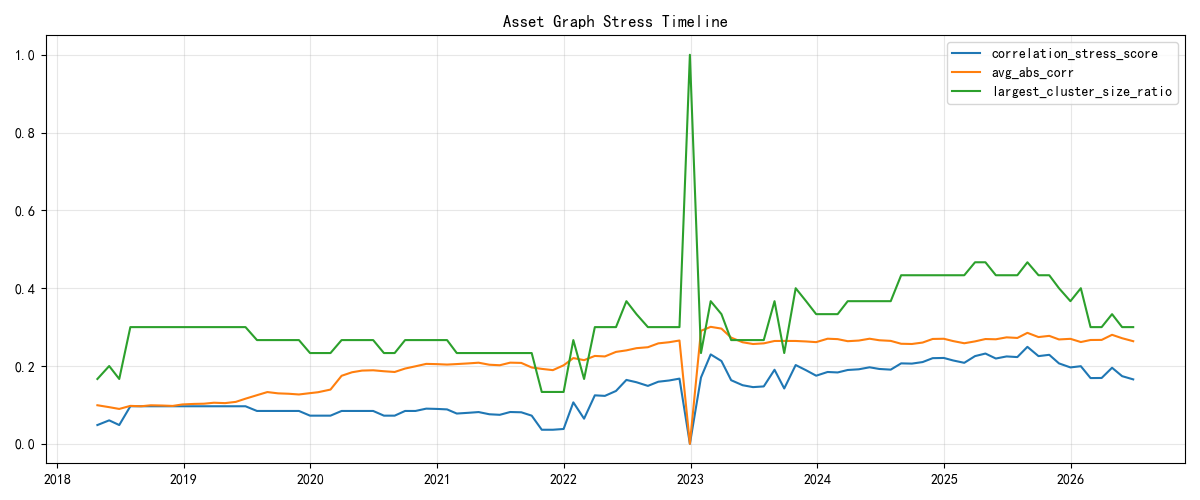
\includegraphics[width=\textwidth,height=0.65\textheight,keepaspectratio]{asset_graph_stress_timeline.png}\\
      \footnotesize\centering 资产层面的压力时序
    \end{column}
  \end{columns}
  \vspace{0.2em}
  \footnotesize\centering
  2020 新冠、2022 加息等主要压力期，Improved Convex 的 CVaR 约束使最大回撤控制在 \improvedMaxDD{} 以内
\end{frame}

% ════════════════════════════════════════════════════════════════════════════
\section{主要结论}
% ════════════════════════════════════════════════════════════════════════════

\begin{frame}{三条核心结论}
  \begin{swufekeypoints}
    \swufepoint{三维权衡同步改善}{01}{Improved Convex 月换手从 \globalMonthlyTurnover{} 降至 \improvedMonthlyTurnover{}，净 Sharpe 升至 \improvedSharpe{}（统计显著，$p=\improvedVsGlobalPValue$），最大回撤收窄至 \improvedMaxDD{}——在收益、回撤、换手三个维度上均无明显短板}
    \swufepoint{HERC 高 Sharpe 不具可比性}{02}{HERC 年化波动率仅 \hercVolatility{}，净收益 \hercNetReturn{}，其 Sharpe = \hercSharpe{} 完全来自接近全仓债券的极低波动，而非跨资产分散的结果，不构成多资产配置框架的有效基准}
    \swufepoint{结论有明确的适用边界}{03}{所有数字均条件于 \evalStartDate{}—\evalEndDate{} 这一特定样本区间和冻结参数设定；Walk-forward 和参数扰动分析确认结论在区间内相对稳定，但不代表对未来绩效的预测}
  \end{swufekeypoints}
\end{frame}

\begin{frame}{研究局限与未来方向}
  \begin{columns}[T]
    \begin{column}{0.48\textwidth}
      \textbf{三项研究局限}
      \begin{enumerate}
        \item \textbf{样本期偏短}：\evalMonths{} 个月，包含低利率→快速加息完整周期，与更长历史均值存在结构性偏差
        \item \textbf{协方差估计滞后}：EWMA 在市场机制快速切换时存在系统性滞后；更先进的估计器尚未纳入
        \item \textbf{成本模型简化}：线性近似在大规模执行场景下忽视了市场冲击和流动性约束
      \end{enumerate}
    \end{column}
    \begin{column}{0.48\textwidth}
      \textbf{未来研究方向}
      \begin{itemize}
        \item[\textcolor{swufeGold}{$\triangleright$}] \textbf{因子层双层预算}：资产层 + 因子层 CVaR 约束联合优化
        \item[\textcolor{swufeGold}{$\triangleright$}] \textbf{深度学习协方差}：端到端估计器与凸优化框架的接口设计
        \item[\textcolor{swufeGold}{$\triangleright$}] \textbf{更长历史区间}：含 2015 股灾、2020 新冠的完整周期验证
        \item[\textcolor{swufeGold}{$\triangleright$}] \textbf{精细化成本建模}：滑点、冲击成本的非线性建模与动态换手策略
      \end{itemize}
    \end{column}
  \end{columns}
\end{frame}

% ════════════════════════════════════════════════════════════════════════════
% 致谢与问答
% ════════════════════════════════════════════════════════════════════════════
\begin{frame}[plain]
  \begin{tikzpicture}[remember picture, overlay]
    \fill[swufeDark] (current page.south west) rectangle (current page.north east);
    \foreach \r in {2.5, 3.8, 5.1}{%
      \draw[swufeGold, opacity=0.15, line width=0.8pt]
        (current page.north east) circle(\r cm);}
    \fill[swufeGold]
      (current page.south west) rectangle ([yshift=6pt]current page.south east);
    \node[text=white, font=\Large\bfseries]
      at ([yshift=0.5cm]current page.center){感谢各位老师的聆听与指导};
    \node[text=swufeGold, font=\normalsize]
      at ([yshift=-0.3cm]current page.center){敬请批评指正};
    \node[text=white!70, font=\scriptsize, anchor=south east]
      at ([xshift=-1.5cm, yshift=1.5cm]current page.south east){
      \begin{tabular}{rl}
        净年化收益 & \improvedNetReturn \\
        Sharpe    & \improvedSharpe    \\
        最大回撤  & \improvedMaxDD     \\
        月均换手  & \improvedMonthlyTurnover \\
      \end{tabular}};
    \node[anchor=north west, opacity=0.6, inner sep=0pt, outer sep=0pt]
      at ([xshift=1cm, yshift=-0.8cm]current page.north west){%
      
\includegraphics[height=1.2cm]{logo.png}};
  \end{tikzpicture}
\end{frame}

\end{document}
